\chapter{Quellen und Methoden}\label{sec:Quellen}

Das im Rahmen dieser Arbeit bearbeitete Quellenmaterial umfasst 10\,519 Fundstücke von 122 individuellen Fundplätzen in einem 500\,$\times$\,700\,km großen Arbeitsgebiet (siehe Kap.~\ref{sec:Arbeitsgebiet}). Das Material stammt zu einem großen Teil aus 143 differenzierten Komplexen von Oberflächenabsammlungen. Eine belastbare Quellenbasis bildeten 13 ausgegrabene sowie sechs weitere, zwar als Befunde erkannte, aber nicht systematisch untersuchte Komplexe (Tab.~\ref{TabBefundeUntersucht}). Im Anschluss an die Feldarbeiten wurde mit der Aufarbeitung der Funde begonnen. Die in Hamburg durchgeführten Arbeiten umfassten neben der Restaurierung und Beschriftung der Keramik auch die Anfertigung von Fundzeichnungen. Überdies wurden in den 2000er Jahren in Tübingen weitere Abbildungen der Gefäßkeramik erstellt.\footnote{Die von Rita Vollbracht (Hamburg) erstellten Keramikzeichnungen bildeten den Grundstock der Fundtafeln. Die Erstellung der in kombinierter Ansicht erstellten Abbildungen oblag Stefanie Samida und Michele Williams-Schmid (beide ehem. Tübingen).}

Da zum Beginn der Arbeit keine geografischen Koordinaten der zu bearbeitenden Fundstellen bekannt waren, mussten diese nachträglich ermittelt werden. Die Lokalisierung der Fundstellen und ihrer Koordinaten wurde durch Abgleich von während der Befahrungen der Flüsse geführten Flussatlanten mit GoogleEarth-Satellitendaten vorgenommen. Diese Vorgehensweise bedingt eine gewisse Unschärfe der ermittelten Positionen, da es von Fall zu Fall kleinere Unterschiede im Kartenmaterial gab. Die Positionen der Fundstellen innerhalb der Ortschaften ließ sich nicht präziser rekonstruieren.\footnote{Die in GoogleEarth ermittelten Koordinaten für die Fundstellen wurden in Dezimalgrad umgerechnet und als Längen- sowie Breitenangabe in die Datenbank übernommen (Abb.~\ref{fig:DB-Schema}).} Die Vergabe von Katalognummern, im weiteren als \enquote*{Fpl.} abgekürzt, schließt an den 185 Fundstellen umfassenden Katalog von \textcite[542f. Karte 1]{Wotzka.1995} an.

Aufgrund des zeitlichen Abstandes zwischen den Feldarbeiten des \textit{River Reconnaissance Project} in den 1980er Jahren und der aktuellen Aufarbeitung konnten offene Fragen an die ursprüngliche Dokumentation nicht immer zufriedenstellend geklärt werden. Als zentrales Problem erwies sich das Fehlen der schriftlichen Felddokumentation von Célestin Kanimba Misago, dem damaligen Mitarbeiter des \textit{Musées Nationaux du Zaïre} (heute \textit{Institut des Musées Nationaux du Congo}) in Kinshasa und Kooperationspartner. Während die Feldbücher der übrigen Teilnehmer der Reisen von 1985 und 1987 im Original wie in Kopie vorlagen, konnten jene von Kanimba Misago nicht aufgefunden werden. Während der Kampagne von 1987 hatte Kanimba Misago die Komplexe BBS~87/1 (Kat.-Nr.~6) in Bobusa am unteren Sangha (Fpl.~239) und PIK~87/3 (Kat.-Nr.~10) in Pikunda am mittleren Sangha (Fpl.~255) ausgegraben. Insbesondere im Fall des Metallurgie-Befund PIK~87/3 konnten durch das Fehlen der Dokumentation entscheidenden Schlüsse für die Interpretation des Befundes nicht gezogen werden. Der Befund ist nach Ausweis der vorliegenden Radiokohlenstoffdatierung, welche ihn in das 11.--13.~Jh.~n.~Chr. (Abb.~\ref{fig:PIK87_Datierungen}) datieren, einer der ältesten Belege für einen flachen, offenen Ofen mit Schlackeabfluss in Zentralafrika. Da auch keine Zeichnungen vorhanden sind, basieren die gewonnenen Erkenntnisse ausschließlich auf einer nur bedingt systematischen fotografischen Dokumentation (Details siehe Kat.-Nr.~10).

Die angesprochene Aktenlagen umfasste neben der ursprünglichen Dokumentation, die im Gelände angefertigt wurde, auch eine Reihe von internen Berichten und Teile unveröffentlichter Manuskripte. Wo diese für die Aufarbeitung des Materials herangezogen wurden, sind sie entsprechend als Quelle im Text ausgewiesen. Die in dieser Arbeit durchgeführten Analysen gründen sich in allen Fällen jedoch auf die eigenen Beobachtungen des Autors am Fundmaterial sowie der Auswertung der im Gelände angefertigten Dokumentation (Katalog~A).

\section{Surveys, Grabungen und Befunde}\label{sec:GrabungenBefunde}

\subsection{Grubenbefunde}

In die Auswertung flossen 13 Grabungsbefunde ein sowie sechs Komplexe, die zwar einen klaren Befundcharaktere aufweisen, aber nicht systematisch ergraben wurden (Tab. \ref{TabBefundeUntersucht}). Zur letzteren Gruppe werden zum Beispiel die beiden Komplexe MLB~85/103 (Kat.-Nr.~5) und LKW~87/186 (Kat.-Nr.~19) gerechnet, die zwar eindeutig als Gruben angesprochen werden können, jedoch nicht ausgegraben wurden. Da sich diese Gruppe von Befunden aber aufgrund ihrer Geschlossenheit grundsätzlich von den ebenfalls in die Gesamtauswertung eingeflossenen Surveyfunden unterscheidet, werden sie der Kategorie der \enquote*{Befunde} zugerechnet. Die 13 ergrabenen Befunde stammen aus fünf verschiedenen Fundstellen.

\begin{table*}[!b]
\centering
%\resizebox{\textwidth}{!}{%
{\small
\begin{tabular}{@{}lllll@{}}
\toprule
\textbf{Fundstelle} & \textbf{Gruben} & \begin{tabular}[c]{@{}l@{}}\textbf{Metallurgie-}\\ \textbf{befunde} \end{tabular} & \textbf{Gräber} & \begin{tabular}[c]{@{}l@{}}\textbf{\enquote*{Schichten}-}\\ \textbf{Abfolge} \end{tabular} \\
\midrule
\begin{tabular}[c]{@{}l@{}}\textbf{Maluba}\\(Fpl.~230)\end{tabular} & \begin{tabular}[c]{@{}l@{}}MLB 85/1-3-1\\ MLB 85/1-3-2\\ (MLB 85/2)\\ (MLB 85/103)\end{tabular} & & MLB 85/1-4-3 & \\ %\hdashline
\begin{tabular}[c]{@{}l@{}}\textbf{Bobusa}\\(Fpl.~239)\end{tabular} & & & & \begin{tabular}[c]{@{}l@{}}BBS 87/1\\ BBS 87/2\end{tabular} \\[3ex] %\hdashline
\begin{tabular}[c]{@{}l@{}}\textbf{Pikunda}\\(Fpl.~255)\end{tabular} & \begin{tabular}[c]{@{}l@{}}PIK~87/1\\ PIK~87/2\end{tabular} & PIK~87/3 & & \\[3ex] %\hdashline
\begin{tabular}[c]{@{}l@{}}\textbf{Ngombe}\\(Fpl.~252)\end{tabular} & (NGO~87/102) & & & \\[3ex] %\hdashline
\begin{tabular}[c]{@{}l@{}}\textbf{Mitula}\\(Fpl.~251)\end{tabular} & (MIT~87/103) & & & \\[3ex] %\hdashline
\begin{tabular}[c]{@{}l@{}}\textbf{Mobaka}\\(Fpl.~246)\end{tabular} & (MKA~87/102) & & & \\[3ex] %\hdashline
\begin{tabular}[c]{@{}l@{}}\textbf{Boleko}\\(Fpl.~285)\end{tabular} & & & BLK 87/1 & \\[3ex] %\hdashline
\begin{tabular}[c]{@{}l@{}}\textbf{Likwala Fluss-}\\ \textbf{Kilometer~186}\\(Fpl.~291)\end{tabular} & (LKW~87/186-1) & & & \\[3ex] %\hdashline
\begin{tabular}[c]{@{}l@{}}\textbf{Munda}\\(Fpl.~304)\end{tabular} & \begin{tabular}[c]{@{}l@{}}MUN~87/2-1-1 A \\ MUN~87/2-1-3\end{tabular} & \begin{tabular}[c]{@{}l@{}}MUN~87/1 \\ MUN~87/2-1-1 B/C \\ MUN~87/3\end{tabular} & & \\
\bottomrule
\end{tabular}}
%}
\caption{Ausgegrabene Befunde: Übersicht über die untersuchten Befunde im Arbeitsgebiet aufgeteilt nach Befundkategorien. Die in Klammern stehenden Komplexe wurden nicht systematisch ausgegraben, aber als Befunde erkannt. Die Sortierung der Liste orientiert sich an der Abfolge, in der die Befunde untersucht wurden.}
\label{TabBefundeUntersucht}
\end{table*}

Im Jahr 1985 wurden bei der Befahrung der Flüsse Ubangi und Lua lediglich in Maluba am Lua (Fpl.~230, Kat.-Nr.~1--5) Grabungen durchgeführt. Von den insgesamt vier dort ausgegrabene Gruben wurden nur zwei vollständig untersucht und dokumentiert (Kat.-Nr.~1--2). Die ursprüngliche Verfüllung einer weiteren Grube (Kat.-Nr.~4) stürzte während der Grabung ein. Daher wurde der Befund nicht mehr weiter untersucht. Es wurden auch keine Funde dieses Befundes geborgen beziehungsweise zur Auswertung lagen keine Funde aus dieser Grube mehr vor. Eine vierte Grube (Kat.-Nr.~5) ist zwar als solche zu erkennen gewesen, es wurde aber lediglich eine geringe Menge keramischen Fundgutes entnommen und keine Ausgrabung durchgeführt. Während der Kampagne von 1987 im nördlichen Teil der Republik Kongo, entlang der Flüsse Sangha, Ngoko und Liwkala-aux-Herbes sowie eines kurzen Abschnitts des Kongo, wurden zehn Befunde an vier verschiedenen Fundstellen untersucht. In Pikunda am mittleren Sangha (Fpl.~255) wurden an zwei benachbarten Grabungsstellen insgesamt drei Gruben (Kat.-Nr.~8--9) erfasst. In Munda am Likwala-aux-Herbes (Fpl.~304) fanden die umfangreichsten Ausgrabungen des \textit{River Reconnaissance Project} im Arbeitsgebiet statt. Innerhalb eines eng begrenzten Areals wurden vier Komplexe näher untersucht, die drei Gruben sowie drei Verhüttungsbefunde erbrachten. Die Grabungen MUN~87/1 (Kat.-Nr.~15) sowie MUN~87/2--1--1 (Kat.-Nr.~16) ergaben jeweils eine Grube sowie einen Verhüttungsbefund, während es sich bei Befund MUN~87/2--1--3 (Kat.-Nr.~17) um eine weitere Grube handelt.

Für das Sangha- und Likwala-aux-Herbes-Gebiet lassen sich auf Basis der ausgegrabenen Befunde in Pikunda (Fpl.~255) und Munda (Fpl.~304) Grundlagen der chronologischen Sequenz erarbeiten (siehe Kap.~\ref{sec:SequenzLikwala}--\ref{sec:SequenzSanghaNgoko}). Grabungen im Ubangi- und Lua-Gebiet fanden hingegen ausschließlich in Maluba am Lua (Fpl.~230) statt. Sie decken nur eine der belegten keramischen Stilgruppen ab und ermöglichen kaum weiterführende Aussagen zum Ablauf der Besiedlung in der Region. Zwar liefern die Funde aus ausgegraben Kontexten oder eindeutig ansprechbaren Befunden die beste Datenlage, jedoch spiegeln sie nur sehr begrenzte Nutzungsphasen innerhalb der jeweiligen Fundstelle wider.

Das es sich bei dem Gros der ausgegrabenen Befunde um Gruben handelt, spiegelt die archäologische Situation im Arbeitsgebiet und darüber hinaus in ganz Zentralafrika wider, in dem Gruben die am reichhaltigsten belegte Befundkategorie darstellen. Die daraus abzuleitende Frage nach der Bedeutung dieser Befunde, bezogen auf ihre Nutzung und Funktion in der Vergangenheit, ist Gegenstand einer konstanten Diskussion \parencite[siehe][197--199]{Meister.2008b}. Während Merkmale wie die häufig in den Befunden beobachtete fragmentierte Gefäßkeramik sowie botanischen Reste vordergründig eine profane Nutzung nahelegen, deuten andere Eigenschaften andere Nutzungen an. Der bislang ambitionierteste Interpretationsansatz stammt von H.-P. \textcite{Wotzka.1993} und gründet auf der Feldarbeit des \textit{River Reconnaissance Project} sowie einem detaillierten Survey ethnologischer Literaturbelege. Die von Wotzka bearbeiteten 34 Grubenbefunde des Inneren Kongobeckens und die dabei beobachteten Deponierungen von Gefäßkeramik in ihnen bildeten die Grundlange für die Auseinandersetzung mit der Frage nach der Funktion von Keramikdeponierungen in Gruben im zentralafrikanischen Regenwald. \textsc{Wotzka} (ebd. 262f. Tab.~1) stellte die an den Grubenbefunden beobachteten Merkmale zusammen und beschrieb sie im Sinne einer polythetischen, sich aus überschneidenden Typen zusammensetzenden Gruppe \parencite[siehe][37f. mit Abb.~3]{Clark.1968}. Aus archäologischer Perspektive kann er deutlich machen, dass es sich bei den von ihm untersuchten Befunden weder um reine \mbox{Abfall-,} Vorrats-, Lehmentnahme- oder Lateritentnahmegruben handelt \parencite[264]{Wotzka.1993}. Dieser Umstand veranlasste ihn im Weiteren zu einem \enquote{bedingt systematischen} (ebd.~266) Survey ethnografischer Berichte. Ein Fokus der Sichtung der ethnografischen Berichte bildete die an der Gefäßkeramik aus den Gruben beobachtbaren Modifikationen oder intentionellen Zerstörungen von Böden oder Appliken (ebd.~262f. Tab.~1 Merkmale 6, 13 und 15). In seiner abschließenden Bewertung steht für \textcite[272]{Wotzka.1993} die \enquote{Erkenntnis, dass es zahlreiche in rezenter und subrezenter Zeit beobachtete Belege für rituelle Zerstörung von Keramik und anderen Sachgütern gibt, die in einem allgemeinem Zusammenhang mit dem Totenkult stehen}.

% >> Zusätzlich zu den an anderen Fundstellen für die Untersuchung des Fragenkomplexes nach Nutzung und Funktion der Gruben im zentralafrikanischen Regenwald herangezogenen geochemischen Untersuchungen, allen voran die Diskussion von Phosphoranreicherungen an Grubensohlen \parencites[722--724]{MbidaMindzie.19951996}{MbidaMindzie.1998}[App.~2]{Eggert.2016}, soll im späteren Verlauf ein zusätzlicher Untersuchungsansatz diskutiert werden, in welchem Fokus auf der Fragmentierung der in den Befunden angetroffenen Funde liegt (siehe Kap.~\ref{sec:}).\todo{Verweis?}{}

\subsection{Sonstige Befunde}

Neben den Gruben umfasst der Korpus der archäologisch untersuchten Befunde im Arbeitsgebiet noch vier weitere Befunde, die im Allgemeinen als Verhüttungsstrukturen anzusprechen sind und mit der Metallurgiegeschichte der Region in Zusammenhang gebracht werden können (Tab.~\ref{TabBefundeUntersucht}). Einer dieser Befunde wurde in Pikunda am Sangha, zusätzlich zu den genannten Gruben, als dritte Grabungsstelle erfasst (Kat.-Nr.~10). Die drei übrigen Befunde dieser Kategorie wurden ebenfalls 1987 bei den Ausgrabungen in Munda am Likwala-aux-Herbes untersucht. Neben den in den beiden Grabungsstellen MUN~87/1 (Kat.-Nr.~15) sowie MUN~87/2-1-1 (Kat.-Nr.~16) erfassten Verhüttungsstrukturen wurde in unmittelbarer Nähe eine weiter Ofenbefund beobachtete und unter der Befundnummer MUN~87/3 (Kat.-Nr.~18) untersucht.

Zusätzlich zu den genannten Verhüttungsbefunden wurden zwei Bestattungen erfasst. Bei der Grabung im Jahr 1985 in Maluba am Lua (Fpl.~230) wurde zwischen den beiden ausgegrabene Gruben (Kat.-Nr.~1--2) eine in einer kleinen Eingrabung angelegte Sekundärbestattung (Kat.-Nr.~3) erfasst und dokumentiert. Ein subrezentes Körpergrab (Kat.-Nr.~14) wurde 1987 in Boleko am Likwala-aux-Herbes (Fpl.~285) archäologisch untersucht.

Zwei zur Erfassung der jeweiligen \enquote*{Schichtabfolgen} angelegte Sondageschnitte in Bobusa an der Mündung des Sangha (Fpl.~239) wurden ausgehend von bestehenden Bodeneingriffen angelegt. Sie waren jeweils nur 1\,m\textsuperscript{2} groß und reichten nur bis in etwa 1\,m Tiefe (Kat.-Nr.~6--7).


\subsection{Surveys}

Etwa zwei Drittel der untersuchten Funde stammen von Oberflächenabsammlungen. Zusammengenommen konnten 143 separate Komplexe von 118 Fundstellen herangezogen werden. Da die ausgegrabenen Befunde nur einen ungenügenden Einblick in die chronologischen Relationen zwischen den keramischen Stilgruppen boten und somit eine Rekonstruktion des Besiedlungsganges auf Basis dieser Daten nicht möglich war, musste dem von der Oberfläche der Dörfer abgesammelten Material verstärkt Beachtung geschenkt werden. Die Inventare aus Oberflächenabsammlungen setzen sich im Mittel aus jeweils gerade einmal 40 Fundstücken zusammen. Während die umfangreichsten Komplexe aus bis zu 289 Stücken bestehen, setzt sich die Hälfte aller Komplexe aus Oberflächenabsammlungen aus weniger als 22 Fundobjekten zusammen. Neben den grundsätzlichen Schwierigkeiten im Umgang mit Funden aus Oberflächensurveys illustrieren die genannten statistischen Kennzahlen die Probleme bei der quantitativen Auswertung der entsprechenden Komplexe.

Die interne Zusammensetzung von Komplexen aus Oberflächensurveys ist grundsätzlich vielfältigen Parametern unterworfen.\footnote{Die Zusammensetzung eines Komplexes aus einem Oberflächensurvey ist nur zum Teil durch die archäologische sowie geomorphologische Situation an der Fundstelle bestimmt. In den hier zur Untersuchung vorliegenden Funden aus Dörfern im Zentralafrikanischen Regenwald ist aufgrund der gängigen Praxis des Fegens der Dorffläche zur Reinhaltung vor Bewuchs und Kleintieren mit einer großen Verlagerung von Objekten innerhalb der Fundstelle zu rechnen. Darüber hinaus spielen aber auch Faktoren eine Rolle, die mit dem Survey selbst zu tun haben, wie die Witterung, die Nutzung spezifischer Bereiche eines Dorfes zum Zeitpunkt des Surveys und auch die Erfahrung des Sammelnden.} Indizien für eine mögliche Vermischung von Funden ergaben sich im Zuge der Auswertung der Survey-Inventare von zwei im Gelände unterschiedenen Bereiche einer Fundstelle. Im Fall von zwei anderen Inventaren wurde eine Vermischung der Funde bereits 1990 festgestellt.\footnote{Aus Bobusa am unteren Sangha (Fpl.~239) liegen zwei direkt anpassende Scherben eines Reiseherdes vor (siehe Kap.~\ref{sec:Reiseherde}). Während ein Stück im Dorf (BBS~87/101:10) gefunden wurde, stammt eine weiteres, direkt anpassendes Fragment aus dem \textit{elali}\footnote{Dorfwüstungen werden als \textit{bilali}; im Singular \textit{elali} bezeichnet.} (BBS~87/102:81). Dieses soll nach den Angaben im Feldbuch Manfred Eggerts etwa 7 Weg-Minuten vom Dorf entfernt gelegen haben. Auf Basis der vorliegenden Unterlagen kann eine simple Verwechslung der Nummerierung bei der Beschriftung der Stücke im Anschluss an die Feldkampagne von 1987 nicht ausgeschlossen werden. In wie weit eine mögliche Verlagerung der Funde auf natürlichem oder artifiziellem Wege bestehen kann, muss offen bleiben. Das Material des Komplexes NGO~87/101 aus Ngombe am Sangha (Fpl.~252) wurde zu einem nur grob eingrenzbaren Zeitpunkt mit jenem des Komplexes NGL~87/101 aus Ngombe am Likwala-aux-Herbes (Fpl.~283) vermischt. Allen Funde des Komplexes NGO~87/101 wurde die Kennung NGL~87/101 gegeben. Erkannt wurde dieser Umstand erst 1990 von Eggert, als bei einer Durchsicht der Funde der Kampagne von 1987 auffiel, dass \enquote*{offiziell} keine Funde mit der Kennung NGO 87/101 vorliegen. Im Fall der Scherben aus den beiden Fundstellen muss die Vermischung bereits sehr zeitig, möglicherweise bereits im Feld, bei der Vorbereitung des Exports der Funde, oder kurz danach stattgefunden haben. In den verfügbaren Packlisten waren bereits nur die beiden Komplexe NGL~87/101 und NGO~87/102 und kein Komplex NGO~87/101 verzeichnet. Ein entsprechender Komplex ist jedoch eindeutig im Feldbuch Eggerts sowie der Kartei der Fundstellenkürzel mit der Beschreibung \enquote{Dorf allgemein} ausgewiesen. Im Zuge der Aufarbeitung der Funde ergaben sich keine stichhaltigen Indizien, die eine Trennung des mit NGL~87/101 beschrifteten Materials, insgesamt 112 Scherben, auf zwei Komplexe ermöglichte. Auffällig ist lediglich das Auftreten von rouletteverzierter Keramik, die an Fundstellen entlang des Likwala-aux-Hebers kaum beobachtet wurde (siehe Kap.~\ref{sec:SequenzLikwala}), am Sangha jedoch durchaus vertreten ist (siehe Kap.~\ref{sec:SequenzSanghaNgoko}). Aus dieser Beobachtung ließ sich jedoch keine Regelmäßigkeit ableiten. Die Keramik wurde folglich nicht in die Auswertung integriert.\label{ftn:Vermischungen}}


\section{Funde}

Die umfangreichste Fundgattung innerhalb des untersuchten Materials bildet die Gefäßkeramik (Tab.~\ref{tab:Funde_Übersicht}). Insgesamt 8469 Gefäßeinheiten und Scherben machen 80\,\% des gesamten Fundgutes aus. Unter den restlichen, nichtkeramischen Funde nehmen Metallurgieüberreste, vor allem Schlacken mit 1321 Stücken beziehungsweise knapp 40\,kg eine hervorzuhebende Stellung ein. Die weiteren Fundkategorien sind häufig nur durch wenige Stücke vertreten (Tab.~\ref{tab:Funde_Übersicht}).

\begin{table*}[tb]
\centering
{\small \input{output/tabs/2-2_Funde_modDS}}
\caption{Funde: Übersicht der in die Auswertung eingeflossenen Fundkategorien und ihrer Anteile.}
\label{tab:Funde_Übersicht}
\end{table*}

\begin{figure*}[tb]
\centering
\includegraphics[width=.75\textwidth]{output/figs/2-2_FundeGewicht_FlussKM_2.pdf}
\caption{Funde: Vergleich des Fundaufkommens (rot) mit Bezug auf die Länge des befahrenen Flussabschnitts (blau).}
\label{fig:FundGewVSFlussKM}
\end{figure*}

Die Funde sind, obschon der Geländearbeit innerhalb beider Kampagnen die gleiche Surveystrategie zugrunde lag, nicht gleichmäßig im Arbeitsgebiet verteilt. Während einigen Regionen sehr gut repräsentiert sind, liegen aus anderen Räumen nur vergleichsweise wenige Funde vor. Besonders deutlich wird dies bei einer Gegenüberstellung des Fundaufkommens von den drei größten, befahrenen Flüsse: Ubangi, Sangha und Likwala-aux-Herbes (Abb.~\ref{fig:FundGewVSFlussKM}). Die Funde vom Ubangi, der noch in der zweiten Hälfte der Feldkampagne von 1985 befahren wurde, machen weniger als 20\,\% des gesamten Fundmaterials aus, während die etwa 850\,km befahrene Strecke (Tab.~\ref{tab:ArbeitsgebietFlussstrecken}) knapp 40\,\% der in die Untersuchung eingeflossenen Flusskilometer entspricht. Die Prospektion entlang des Ubangi repräsentiert den längsten Transekt durch das Arbeitsgebietes, vom Zentrum des äquatorialen Regenwaldes nahe Mbandaka bis in die Savannenregionen nördlich von Bangui. Genau gegenteilig stellt sich das Verhältnis im Fall des Likwala-aux-Herbes dar (Abb.~\ref{fig:FundGewVSFlussKM}): das Fundmaterial von diesem Fluss macht mit etwa 47\,\% knapp die Hälfte aller Funde aus, während die 500\,km befahrene Flusskilometer nur etwa 23\,\% der insgesamt befahrenen Flusskilometer entsprechen. Der Anteil der Funde vom Sangha entspricht mit etwa 25\,\% dem Anteil der befahrenen Flussstrecke von 27\,\%. Die Funde aus dem befahrenen Gebieten entlang der Flüsse Lua, Ngoko und Kongo/Zaïre nehmen hingegen einen deutlich marginalen Anteil am Gesamtbestand ein. Allerdings gingen die Befahrungen dieser Flüsse nie über 100\,km hinaus (Tab.~\ref{tab:ArbeitsgebietFlussstrecken}) und von den jeweiligen Flüssen liegen lediglich zwischen 4 und 10 Komplexen vor. Sie nehmen in allen Betrachtungsweisen folglich nur eine nachrangige Stellung ein. In der Gesamtschau werden die Erkenntnisse, die sich aus der Befahrung des Lua ergaben den Informationen vom Ubangi hinzugerechnet, da sich mit Blick auf die Besiedlungsgeschichte entlang des Lua keine eigenständige Entwicklung erkennen ließ (siehe Kap.~\ref{sec:SequenzUbangiLua}). In gleichem Maße werden die Untersuchungsergebnisse aus der Prospektion des Ngoko in direktem Zusammenhang zu den Erkenntnissen vom Sangha diskutiert (Kap.~\ref{sec:SequenzSanghaNgoko}).


\subsection{Gefäßkeramik}\label{sec:GefKeramik}

\begin{figure*}[!tb]
\centering
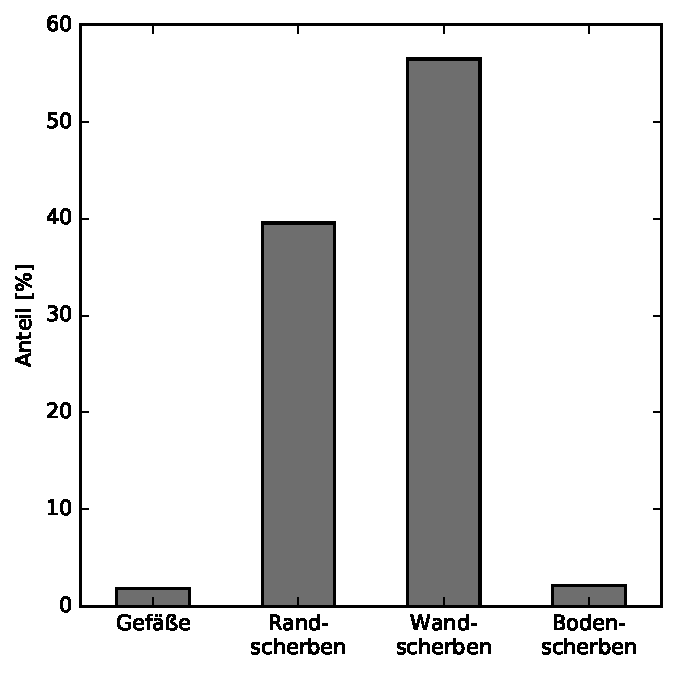
\includegraphics[width=.5\textwidth]{output/figs/2-2-1_KeramikScherbentyp.pdf}
\caption{Keramik: Scherbentypen.}
\label{KeramikScherbentypen}
\end{figure*}

Die aus dem Arbeitsgebiet vorliegende Gefäßkeramik bildet den Grundstock der durchgeführten Analysen. Das Fundgut wurde mittels eines spezifischen Aufnahmesystems, welches sich vor allem an der Aufnahme von \textcite{Wotzka.1995} orientierte und um spezifische Elemente der Arbeiten von \textcites{Nordstrom.1972}{Stehli.1973}{Keding.1997}{Jesse.2003}{Clist.20042005} erweitert wurde, in einer relationalen Datenbank erfasst (siehe Kap.~\ref{sec:Datenhaltung}). Die Systematik der Aufnahme des vornehmlich für die Analyse entscheidenden keramischen Fundmaterials gründet -- in Anlehnung an \textcite[57ff.]{Stehli.1973} -- auf drei Aufnahme- und den sich daraus ergebenden Analyseebenen \parencite[siehe][36]{Keding.1997}:\footnote{Für die Ebenen 2 und 3 gilt die unten stehende Unterscheidung der Gefäßregionen (Abb.~\ref{fig:Keramik_VerzZonen}) in gleichem Maße.}
\begin{enumerate*}
	\item Technologie (Kap.~\ref{sec:Herstellung})
	\item Form (Kap.~\ref{sec:Keramiksequenz})
	\item Verzierung (Kap.~\ref{sec:Keramiksequenz})
\end{enumerate*}

%\vspace{\baselineskip}
\noindent Wann immer möglich wurden aus dem vorliegenden Scherbenmaterial Gefäßeinheiten, im Folgenden GE genannt \parencite[siehe][]{Jesse.2003}, gebildet, die bei der Fundaufnahme im einzelnen beschrieben wurden. Die GE wurden, wenn sich keine direkten \enquote*{objektiven} Anpassungen ergaben, auf Basis eines \enquote*{subjektiven} Eindrucks der Zusammengehörigkeit gebildet (ebd.~81). Dieser Eindruck fußt auf einer Kombination von Formmerkmalen, Abmessungen beziehungsweise Dimensionierung und Verzierungen sowie den technologischen Eigenschaften, genauer dem Scherben der Einzelstücke. Die Definition von GE ist für die statistische und chronologische Auswertung von Keramik unumgänglich, da ein Vorgehen auf Scherben-Niveau zu einer direkten Abhängigkeit beziehungsweise Korrelation der jeweiligen Analyseergebnisse vom Zerscherbtheitsgrad führen würde \parencites[siehe][36f.]{Keding.1997}[nach][483]{Drew.1988}.\footnote{Das keramische Fundgut des Inneren Kongobeckens wurden durch \textcite[38]{Wotzka.1995} in einem entsprechenden System aufgenommen. Eine individuelle Aufnahme umfasste alle auswertbaren Stücke. Scherben wurden zu Gefäßen zusammengefasst, wenn sich direkte Anpassungen oder eine hinreichende Übereinstimmung von Merkmalen ergab. Die Keramik aus den untersuchten Grabungsbefunden (ebd.~302--390 Kat.-Nr.~1--61) wurde um nicht aussagekräftige Stücke reduziert während für die Fundinventare aus Oberflächensurveys nach dem Teilmengenprinzip aussortiert wurden (ebd.~38). Lediglich für einzelne Merkmalskombinationen repräsentative Stücke wurden aufgenommen.}

Das untersuchte keramische Material setzt sich fast ausschließlich aus Wandscherben (56\,\%) und Randscherben (40\,\%) zusammen. Ganze Gefäße (2\,\%) machen ebenso wie Bodenscherben (2\,\%) nur einen verschwindend kleinen Anteil am keramischen Inventar aus (Abb.~\ref{KeramikScherbentypen}). Insgesamt 41\,\% aller Stücke können eindeutig einer keramischen Stilgruppe zugeordnet werden. Bei 25\,\% des Material ist die Zuordnung fraglich, während 33\,\% des Materials keiner Stilgruppe zugewiesen werden kann und als unbestimmt gilt.

Der Anteil an unverzierten Stücke im Vergleich zu jenen GE aus dem untersuchten Materialkomplex, die Verzierungen aufweisen, variiert zwischen den Komplexen aus Oberflächensurveys und jenen aus Grabungen nur leicht. Während unverzierte Stücke in Oberflächenabsammlungen etwa 25\,\% ausmachen, sind es bei den ausgegrabenen Komplexen (Kat.-Nr.~1--19) knapp 29\,\%. Im Anschluss an die Ausgrabungen der beiden Komplexe PIK~87/1 (Kat.-Nr.~8) sowie PIK~87/2 (Kat.-Nr.~9) in Pikunda am Sangha (Fpl.~255) wurde nachweislich unverziertes Scherbenmaterial verworfen. Im vorliegenden und ausgewerteten Fundmaterial dieser beiden Grabungen machen unverzierte Stücke immer noch 26\,\% aller GE aus. Daraus kann gefolgert werden, dass die Selektion der Stücke im Gelände die Repräsentanz der Fundinventares nur teilweise beeinträchtigt hat. Die Grabungen in Maluba am Lua (Fpl.~230; Kat.-Nr.~1--5), für die kein Aussondern \enquote*{un-diagnostischer} Stücke überliefert ist, umfasste hingegen lediglich 18\,\% unverzierte Scherben. Diese Angaben legen nahe, das die Oberflächenabsammlungen, zumindest mit Blick auf das Verhältnis von verzierten zu unverzierten Stücken, nicht grob unrepräsentativ sind.


\subsubsection{Erhaltung}

\begin{table*}[!tb]
\begin{center}
{\small
\begin{tabular}{@{}rll@{}}
\toprule
\textbf{Größe} & \textbf{Zerscherbungsgrad} & \textbf{Fragmentgröße} \\
\midrule
$<$30\,$\times$\,30\,mm & stark & klein \\
$<$70\,$\times$\,70\,mm & mittelstark & mittelgroß \\
$<$120\,$\times$\,120\,mm & gering & groß \\
$<$200\,$\times$\,200\,mm & kaum & sehr groß \\
$>$200\,$\times$\,200\,mm & \begin{tabular}[c]{@{}l@{}}große Gefäßfragmente\\oder ganze Gefäße\end{tabular} & \\
\bottomrule
\end{tabular} }
\end{center}
\caption{Funde: Konkordanz der aufgenommenen Größenklassen \parencite[nach][89]{Clist.20042005} und deren verbale Umschreibung im Text.}
\label{tab:Keramik_Fragemtierung}
\end{table*}

\begin{figure*}[!tb]
\centering
\begin{subfigure}{0.49\textwidth} % Choose 0.49 to prevent minipages stacking
\centering
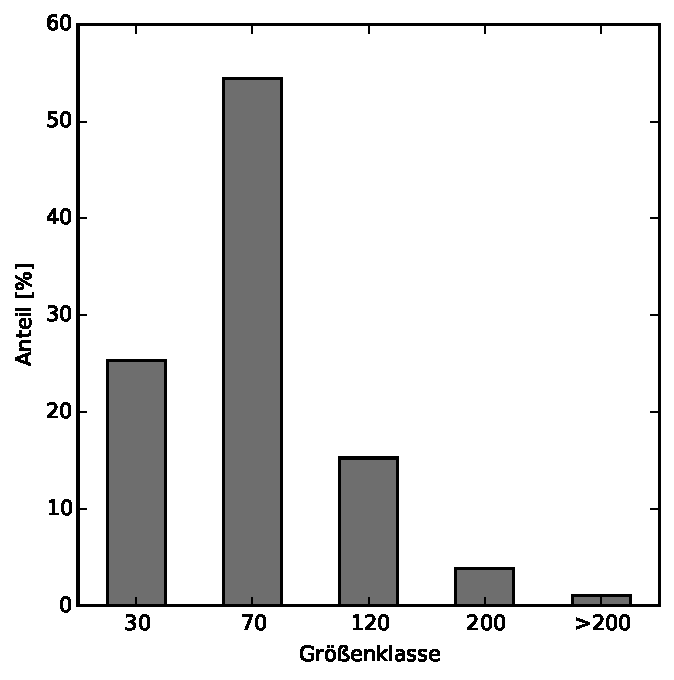
\includegraphics[height=.9\textwidth]{output/figs/2-2-1_KeramikFragmentierung.pdf}
\caption{Fragmentierung der Scherben (Größen-\\klassen siehe Tab.~\ref{tab:Keramik_Fragemtierung}).}
\label{KeramikFragmentierung}
\end{subfigure}
\begin{subfigure}{0.49\textwidth} % Choose 0.49 to prevent minipages stacking
\centering
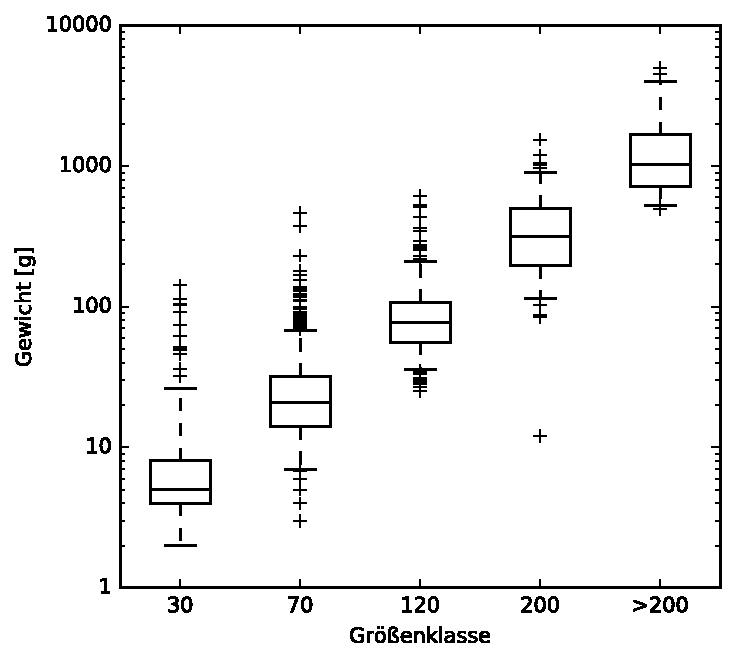
\includegraphics[height=.9\textwidth]{output/figs/2-2_Keramik_Gr-Gew_BoxPlt_2.pdf}
\caption{Verhältnis von Scherbengröße- und gewicht (Größenklassen siehe Tab.~\ref{tab:Keramik_Fragemtierung}; n = 4218).}
\label{fig:Keramik_FragmGrGew_B}
\end{subfigure}
\caption{Funde: Fragmentierung.}
\label{fig:Keramik_Typen-Fragm}
\end{figure*}

Von den insgesamt 4217 aufgenommenen Gefäßeinheiten bestehen nur 654 aus mehr als einer Scherbe. Im Mittel bestehen die Gefäßeinheiten aus etwa 1,5 Scherben, was eine sehr starke Fragmentierung anzeigt und als Indikator für eine schlechte Erhaltung gewertet werden kann \parencite[siehe][86]{Jesse.2003}. Das mittlere Gewicht einer Gefäßeinheit liegt bei knapp 67\,g, das mittlere Gewicht der Einzelscherben bei rund 51\,g.\footnote{Der Unterschied ist wohl einzig auf die stark schiefen Verteilungen zurückzuführen.} Eine Dokumentation der erhalten Anteile von Gefäßprofilen und Randdurchmessern \parencite[siehe hierzu][155ff.]{Claen.2011} erfolgte nicht. Die Fragmentierurng der GE beziehungsweise der Zerscherbtheitsgrad der Keramik wurde unter Nutzung einer Größenklassen-Systematik aufgenommen, welches zuletzt auch bei \textcite[89]{Clist.20042005} zur Anwendung kam (Tab.~\ref{tab:Keramik_Fragemtierung}).\footnote{Im Rahmen der Aufnahme angewandte Einteilung umfasst fünf festen Größenklassen von Stücken jeweils kleiner als 30\,$\times$\,30\,mm, 70\,$\times$\,70\,mm, 120\,$\times$\,120\,mm und 200\,$\times$\,200\,mm Größe sowie allen größeren Stücken (\textsc{Clist}~2004/2005:~89). Dieses Klasseneinteilung wurde auch für das nichtkeramische Fundgut, etwa Schlacken angewandt.} Das ursprünglich auf \textcite[379]{Joukowsky.1980} zurückgehende Schema ist bereits bei \textcite[89]{Clist.20042005} insofern verändert, als das die kleinste Klasse von 25\,mm auf 30\,mm angehoben wurde \parencites[nach][]{Claes.1985}{deMaret.1985}.\footnote{Eine detailliertere Aufnahme der Fragmentierung, mittels zum Beispiel der Ermittlung des maximalen Flächeninhaltes (auf volle cm$^2$ gerundet) eines jeden Stücken, wie von H.-P. Wotzka für das Fundmaterial aus Mbandaka (Grabung 2011) und Iyonda (Grabung 2012) angewandt, wurde nicht verfolgt, da das hier vorliegende Fundmaterial einer Reihe von künstlichen Quellenfiltern unterworfen ist. Anders als bei den neueren Grabungen Wotzkas in der Provinz \textit{Équateur} ab 2010, bei denen grundsätzlich alle Funde aufgehoben wurden, ist bei den hier beschriebenen Grabungen Eggerts aus den 1980er-Jahren nicht das komplette Fundgut aufbewahrt worden. Nur 67\,\% der Keramik aus der Grabungsfläche PIK~87/1 (Kat.-Nr.~8) und 55\,\% der Grube PIK~87/2 (Kat.-Nr.~9) wurden 1987 exportiert. Aufgrund dieses Umstandes, und da der Großteil des Fundgutes ohnehin von Absammlungen der Oberfläche stammt, wurde für die Aufnahme der Fragmentierung ein eher pragmatischer Ansatz verfolgt.} Während etwa 25\,\% der Keramik sehr stark fragmentiert sind -- kleiner als 30\,$\times$\,30\,mm -- sind knapp über die Hälfte der Scherben zwischen 30\,$\times$\,30\,mm und 70\,$\times$\,70\,mm groß (Abb.~\ref{KeramikFragmentierung}). Scherben größer als 70\,$\times$\,70\,mm sind seltener vertreten und machen zusammen nur etwa 20\,\% des Materials aus.

Die fünf Größenklassen bilden die Fragmentierung in einem zufriedenstellenden Maß ab, wie eine Gegenüberstellung mit den individuellen Scherbengewichten ergab (Abb.~\ref{fig:Keramik_FragmGrGew_B}). Trotz Ausreißern zeigen die Verteilungen, dass für jede der Größenklassen ein Gewichtsbereich angegeben werden kann, welcher sich von jenem einer anderen Größenklasse im Interquartilabstand unterscheidet. Überlappungen der Verteilungen stellen sich erst bei Betrachtung der zweifachen Standardabweichung ein (Abb.~\ref{fig:Keramik_FragmGrGew_B}: Antennen).\footnote{Zur Interpretation von Box-Whisker-Plots siehe auch \textcite[81]{Hedderich.2016}. Im Fall von Abb.~\ref{fig:Keramik_FragmGrGew_B} markieren die Whiskers beziehungsweise Antennen die 2-Sigma-Standardabweichung der jeweiligen Verteilungen, während die Box (blau) das untere (25\,\%) sowie das obere Quartil (75\,\%) anzeigt und die Linie (rot) den Median markiert. Wird die einfache Standardabweichung zugrunde gelegt, lässt sich keine Überschneidung der Verteilungen beobachten.} Die Verteilungen zeigen insgesamt eine breite Streuung mit einigen Ausreißern, überlagern sich aber nur im Randbereich.

\subsubsection{Technologie}\label{sec:AufnahmeTechnologie}
%\paragraph{Eigenschaften des \textit{Scherbens}}
%$\;$ \\

\begin{table*}[!tb]
	\begin{center}
		{\small
			\begin{tabular}{@{}llr@{}}
				\toprule
				\textbf{Kürzel} & \textbf{Größenklasse} & \textbf{Durchmesser} \\
				\midrule
				VF & Very Fine & 62--125~$\mu$m \\
				F & Fine & 125--250~$\mu$m \\
				M & Medium & 250--500~$\mu$m \\
				C & Coarse & 500--1000~$\mu$m \\
				VC & Very Coarse & 1000--2000~$\mu$m \\
				\bottomrule
		\end{tabular}}
	\end{center}
	\caption{Keramik: Korngrößen nach der \textit{Wentworth-Grainsize-Scale}.}
	\label{tab:Keramik_PartikelGr}
\end{table*}

\begin{table*}[!tb]
	\begin{center}
		{\small
			\begin{tabular}{@{}lrr@{}}
				\toprule
				\textbf{Klasse} & \textbf{\%} & \textbf{Anzahl je 1\,cm$^2$} \\
				\midrule
				$<$1 & 1--2\,\% & • \\
				wenig & 3--5\,\% & • \\
				mittel & 7--10\,\% & • \\
				viel & 15--20\,\% & • \\
				sehr viel & 25--40\,\% & • \\
				\bottomrule
		\end{tabular} }
	\end{center}
	\caption{Keramik: Anteil nichtplastischer Partikel \parencite[Prozentwerte nach][]{Hodgson.1976}.}
	\label{tab:Keramik_PartikelDichte}
\end{table*}

Zusätzlich zu einer formalen Analyse, die sich auf morphologische wie dekorative Charakteristika der Keramik stützt (siehe Kap.~\ref{sec:Keramiksequenz}), bildet eine tiefgreifende Auseinandersetzung mit technischen Parametern eines der Kernziele der Untersuchung. Hierfür grundlegend war die Einbeziehung von keramik-technischen Parametern in das Aufnahmesystem. Die untersuchten Kriterien gründen vornehmlich auf den Untersuchungen von \textcite{Nordstrom.1972} zu sudanesischer Keramik, welche wiederum Ausgangspunkt der neuen Studie von \textcite{Riemer.2011} zu Material aus der Dakhla-Oase in Ägypten waren, an der sich die hier vorgelegte Untersuchung orientiert. Für die Analyse der technologischen Eigenschaften der Gefäßkeramik wurde ein Katalog aus Aufnahmekriterien formuliert, welcher die folgenden Kenngrößen umfasst:
\begin{itemize*}
	\renewcommand\labelitemi{--}
	\item nichtplastische Partikel
	\begin{itemize*}
		\item Größe (nach \textit{Wentworth-Grainsize-Scale})
		\item Dichte \parencites[Tab.~\ref{tab:Keramik_PartikelDichte}; siehe][32]{Kinne.2009}[nach][]{Hodgson.1976}
		\item Art
	\end{itemize*}
	\item Farbe des Scherben
	\begin{itemize*}
		\renewcommand\labelitemi{--}
		\item Kernfarbe
		\item (Brennfarbe)
		\item Unterteilung des Scherben in Oxidationszonen
		\item Ausbildung der Grenze zwischen Oxidationszonen
	\end{itemize*}
	\item Strukturierung der Oberfläche
\end{itemize*}

\noindent Von zentraler Bedeutung sind die Eigenschaften der im Scherben enthaltenen nichtplastischen Partikel. Diese wurden entsprechend ihrer Größe und Art sowie dem Anteil, in dem sie vorkommen, aufgenommen. Die Größe der Partikel wurden entsprechend der international anerkannten \textit{Wentworth-Grainsize-Scale} \parencite[381 Tab.~1, 388 Abb.~3]{Wentworth.1922} aufgenommen, wobei fünf Größenklassen unterschieden wurden (Tab.~\ref{tab:Keramik_PartikelGr}).\footnote{Die Bestimmung der Größenklassen erfolgte makroskopisch sowie unter Zuhilfenahme einer 10-fach vergrößernden Lupe in Referenz zu einer Korngrößen-Karte der Firma \textit{Precision Core} (Denver).} Die Verrundung und Sortierung der Partikel wurden nicht systematisch aufgenommen. Der Anteil an nichtplastischen Partikeln im Scherben wurde auf Basis einer Vergleichstafel zum Abschätzen von Anteilsklassen ermittelt \parencites[Tab.~\ref{tab:Keramik_PartikelDichte}; ][32]{Kinne.2009}[nach][]{Hodgson.1976}. Die Ansprache der Art der Partikel erfolgte basierend auf makroskopisch sichtbaren Kriterien und den Erfahrungen des Autors.

\begin{table*}[tb]
	%\begin{center}
	\centering
	{\small
		\begin{tabular}{@{}lll@{}}
			\toprule
			\textbf{Code} & \textbf{Farbe} & \textbf{MUNSELL-Wert} \\
			\midrule
			S & schwarz/black & 10 YR 2/1 \\
			G & grau/grey & 10 YR 6/1 \\
			W & weiß/white & 10 YR 8/1 \\
			Bg & beige-ocker/yellow & 10 YR 8/6 \\
			Br & braun/dark reddish brown & 2.5 YR 3/4 \\
			R & rot/red & 2.5 YR 4/8--5/8 \\
			\bottomrule
	\end{tabular}}
	%\end{center}
	\caption{Keramik: Farben der Scherbenoberflächen und -brüche.}
	\label{tab:Keramik_Farbe}
\end{table*}

Zusätzlich zu diesen Eigenschaften der im Scherben beobachtbaren nichtplastischen Partikel erfolgte eine systematische Aufnahme der farblichen Zonierung der Stücke. Die farblichen Abstufungen der Keramik wurde mittels einer fünf Zonen umfassenden Unterteilung der Stücke sowie sechs Farbklassen\footnote{Zur Frage der Nutzung von Farbklassen entgegen der Aufnahme individueller MUNSELL-Farbwerte sei an dieser Stelle exemplarisch auf die Diskussion durch \textcite[38]{Keding.1997} verwiesen.} umfassenden Systematik erfasst (Tab.~\ref{tab:Keramik_Farbe}). Die fünf unterschiedenen Zonen gliedern sich in die äußere und innere Oberfläche des Stücks sowie drei Zonen im Profil beziehungsweise Bruch: den Bereich nahe der Außen- sowie Innenseite sowie der Kernbereich selbst. Die Oberflächenfarbe wurden als \enquote{basic surface colour} nach \textcite[44ff.]{Nordstrom.1972} aufgenommen. Die Ausbildung der Grenze zwischen den farblichen Zonen im Profil wurde in Anlehnung an \parencite[27]{Kinne.2009} umschreibend erfasst.

Die Oberflächenstruktur der Stücke wurde unter Referenz auf eine grobe, subjektive Ansprache -- \enquote*{glatt} -- \enquote*{leicht rau} -- \enquote*{rau} -- erfasst. Die bei der Keramik der Mandombe-Gruppe (Kap.~\ref{sec:MDB-Gr}) beobachtete Schlicker-Rauung der Gefäßunterteile (siehe Taf.~47.24) wurde als entsprechende Eigenschaft der Oberfläche erfasst. Spezifische Behandlungen der Oberfläche, wie Engoben, wurden hingegen gesondert, gemeinsam mit Anhaftungen an den Stücken aufgenommen. Für diese Oberflächenbehandlungen wurde keine Systematik herangezogen, die Beobachtungen wurden verbalisiert in der Datenbank verzeichnet.

Die sich aus diesen technischen Eigenschaften des Scherbens ergebenden Gruppen wurden als \textit{Fabrics} konzeptualisiert und werden später detailliert besprochen (Kap.~\ref{sec:Herstellung2_Fabric}).

%\pagebreak
\subsubsection{Form}

\begin{figure*}[!tb]
	\centering
	\resizebox{\textwidth}{!}{%
		{\footnotesize
\begin{sftabular}{@{}m{.02\textwidth} m{.02\textwidth} *7{>{\centering\arraybackslash}m{.1\textwidth}} m{.25\textwidth} @{}m{0pt}@{}@{}} 
 &  & \multicolumn{7}{c}{\textit{Variante}} &  &  \\
 &  & \textbf{1} & \textbf{2} & \textbf{3} & \textbf{4} & \textbf{5} & \textbf{6} & \textbf{7} & & \\
\multirow{10}{*}{\rotatebox[origin=c]{90}{\textit{Grundform} \hspace{9cm}}} & \textbf{A} & 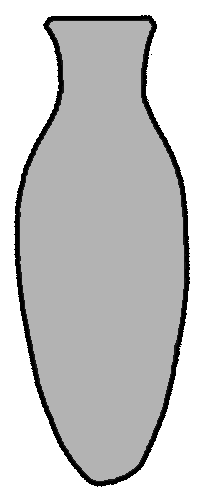
\includegraphics[height=.1\textwidth]{fig/Abb_GefFormen/G11c_Bolongo101.png} & 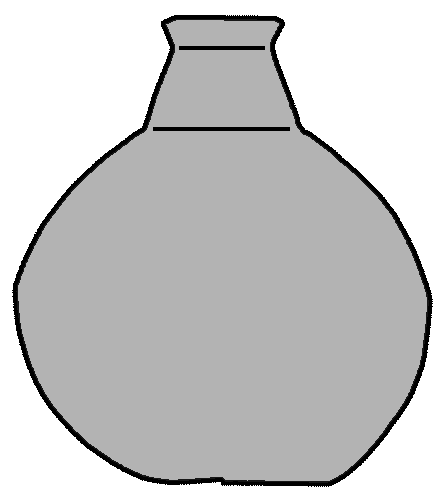
\includegraphics[height=.1\textwidth]{fig/Abb_GefFormen/G11b_MUN87-1-0-2-6-2.png} & 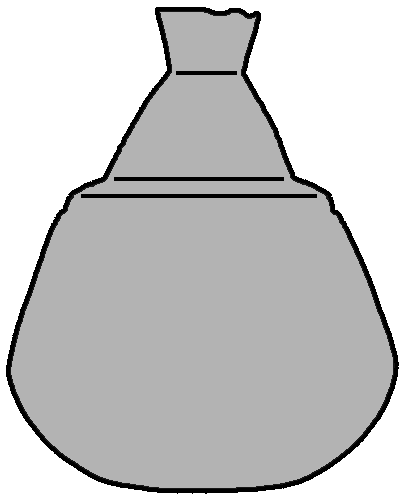
\includegraphics[height=.1\textwidth]{fig/Abb_GefFormen/G11a_MSG87-102-9a.png} &  &  &  &  & Flaschenförmige Gefäße & \\[.11\textwidth]
 & \textbf{B} & 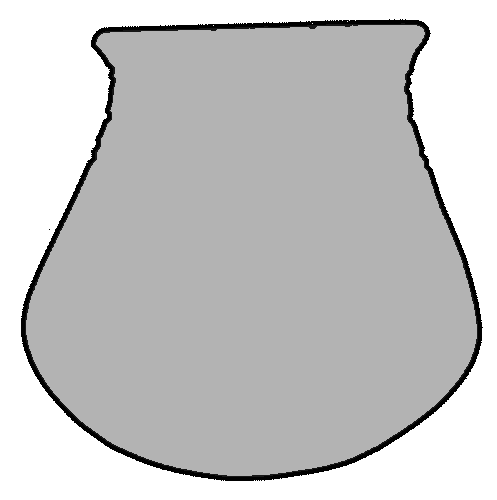
\includegraphics[height=.1\textwidth]{fig/Abb_GefFormen/G5_MUN87-2-1-3-8.png} & 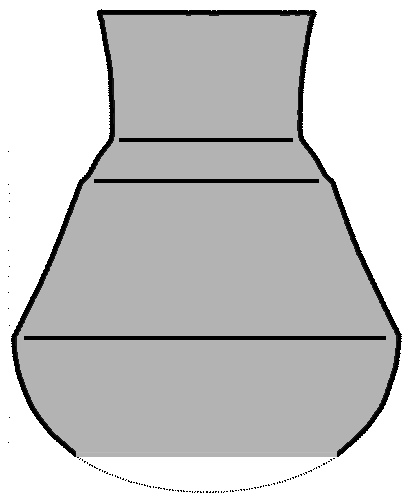
\includegraphics[height=.1\textwidth]{fig/Abb_GefFormen/G6c_msn87-101-145.png} & 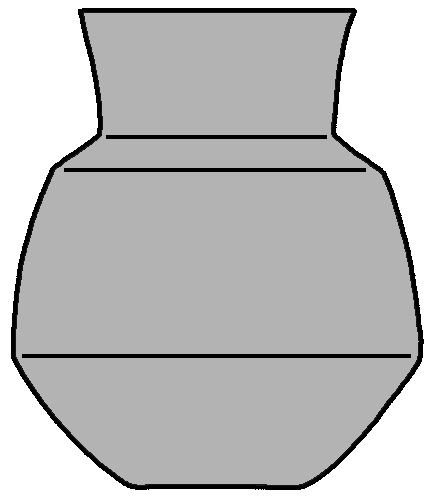
\includegraphics[height=.1\textwidth]{fig/Abb_GefFormen/G6b_ITN87-103-3a.png} & 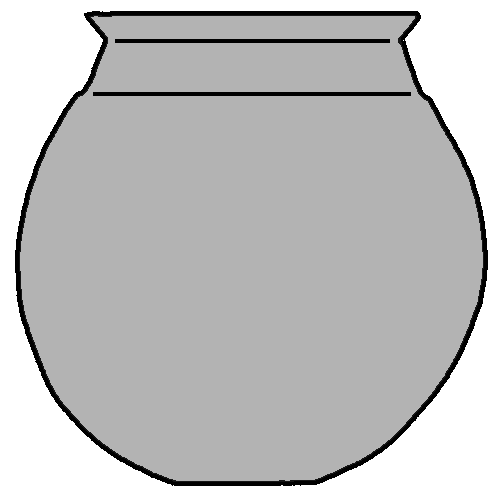
\includegraphics[height=.1\textwidth]{fig/Abb_GefFormen/G6a_MUN87-1-0-2-1.png} & 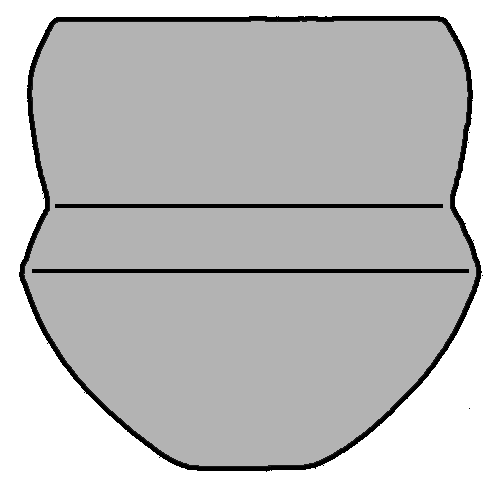
\includegraphics[height=.1\textwidth]{fig/Abb_GefFormen/G13_MKL85-101-114.png} & 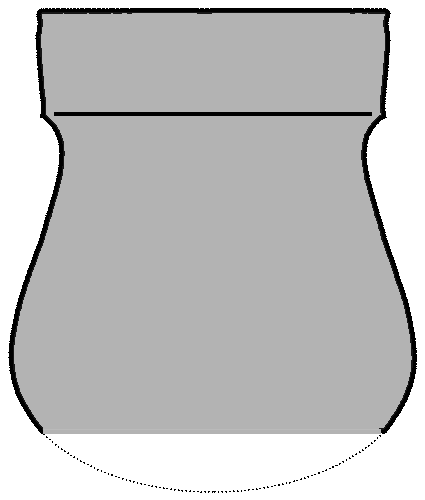
\includegraphics[height=.1\textwidth]{fig/Abb_GefFormen/G4_PIK87-101-51.png} & 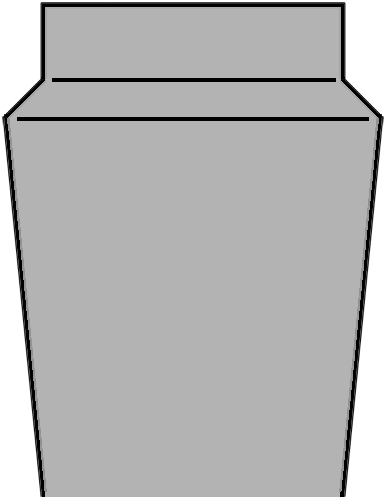
\includegraphics[height=.09\textwidth]{fig/Abb_GefFormen/G4b.png} & hohe Gefäße & \\[.11\textwidth]
 & \textbf{C} & 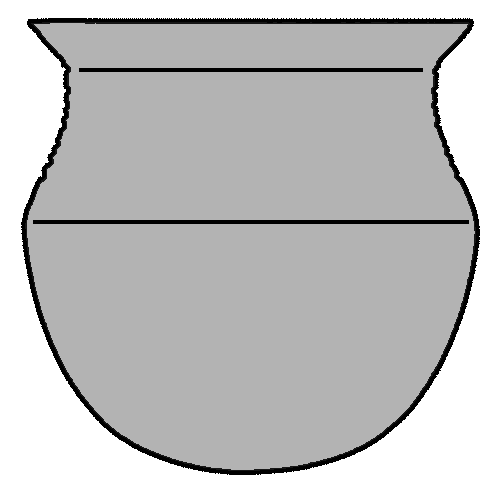
\includegraphics[height=.08\textwidth]{fig/Abb_GefFormen/G7a_NGB85-101-131.png} & 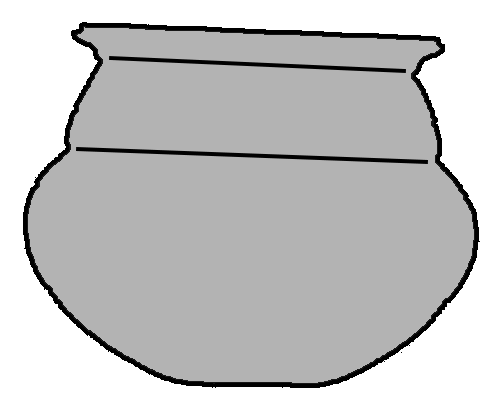
\includegraphics[width=.1\textwidth]{fig/Abb_GefFormen/G7b_DON85-102-a.png} &  &  &  &  &  & Gefäße mit leicht konvexer Wandung und ausgeprägtem Halsbereich & \\[.11\textwidth]
 & \textbf{D} & 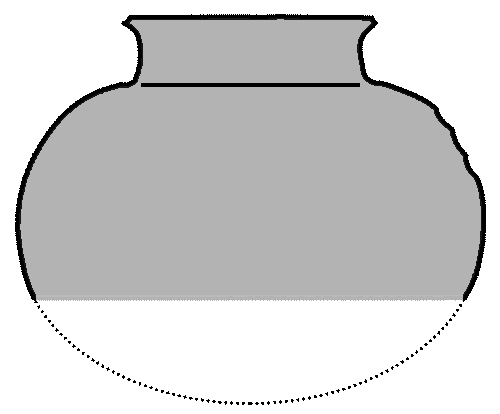
\includegraphics[width=.1\textwidth]{fig/Abb_GefFormen/G7c_PIK87-1-2-3_1-3-7.png} & 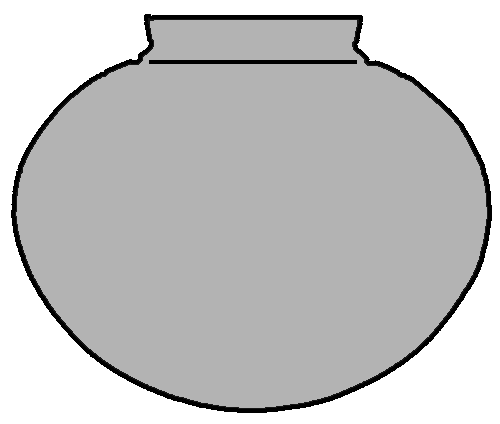
\includegraphics[width=.1\textwidth]{fig/Abb_GefFormen/G10a_NGO87-102-28-29.png} &  &  &  &  &  & Gefäße mit stark konvexer Wandung ohne ausgeprägten Halsbereich & \\[.11\textwidth]
 & \textbf{E} & 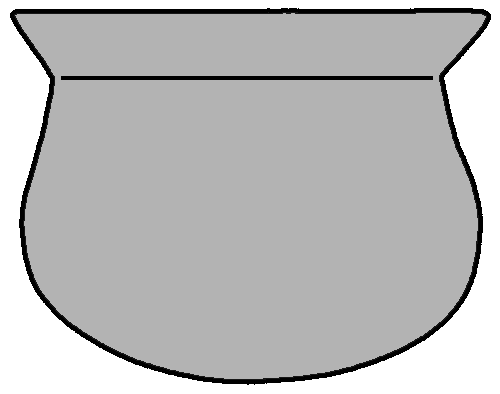
\includegraphics[width=.1\textwidth]{fig/Abb_GefFormen/G3_BLK87-1-1-1-2_HS.png} & 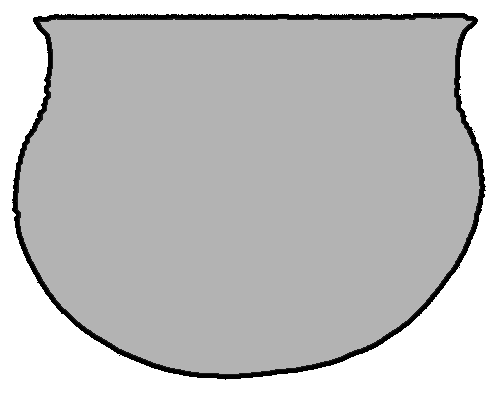
\includegraphics[width=.1\textwidth]{fig/Abb_GefFormen/G3c_MBN85-501-2.png} & 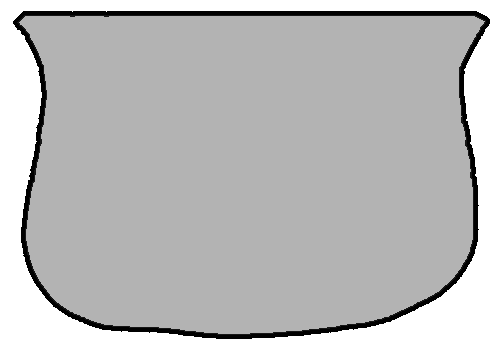
\includegraphics[width=.1\textwidth]{fig/Abb_GefFormen/G1b_MUN87-2-1-3.png} & 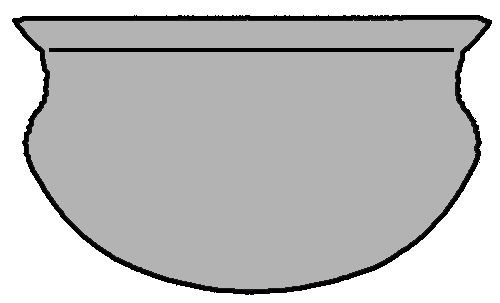
\includegraphics[width=.1\textwidth]{fig/Abb_GefFormen/G8b1_BLN85-201-b.png} & 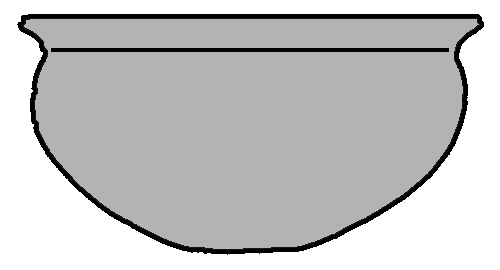
\includegraphics[width=.1\textwidth]{fig/Abb_GefFormen/G9b_DON85-102-b.png} & 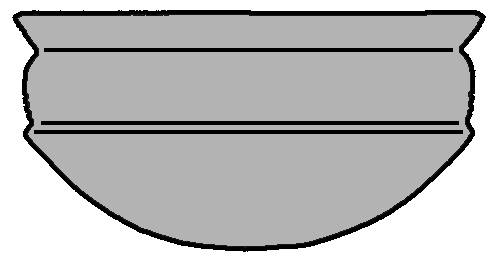
\includegraphics[width=.1\textwidth]{fig/Abb_GefFormen/G2d_SSL87-101-142.png} & 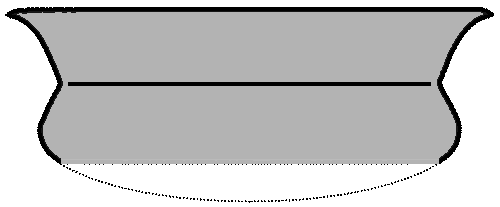
\includegraphics[width=.1\textwidth]{fig/Abb_GefFormen/G3b_GE5_BLK87-1-1-3-1-3.png} & Gefäße mit geschweifter Wandung & \\[.11\textwidth]
 & \textbf{F} & 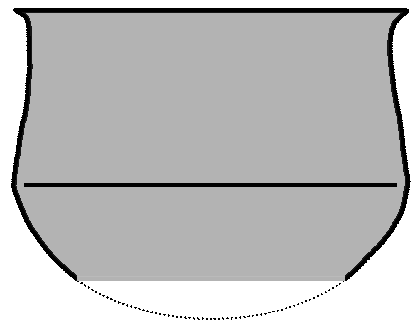
\includegraphics[width=.1\textwidth]{fig/Abb_GefFormen/G1c_LKW87-401-1.png} & 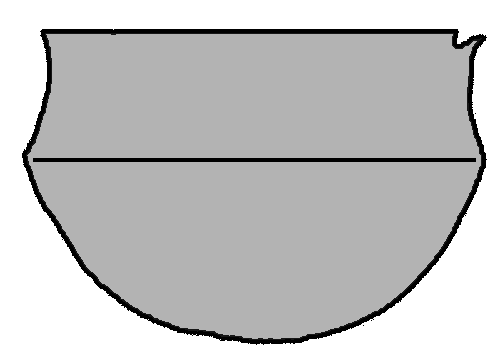
\includegraphics[width=.1\textwidth]{fig/Abb_GefFormen/G1d_MBJ_Roulettekeramik_E87-010-25.png} & 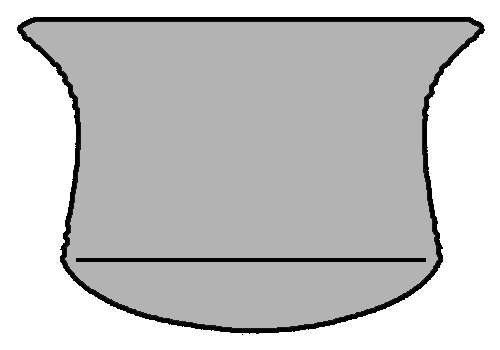
\includegraphics[width=.1\textwidth]{fig/Abb_GefFormen/G1a_PIK87-101-58.png} & 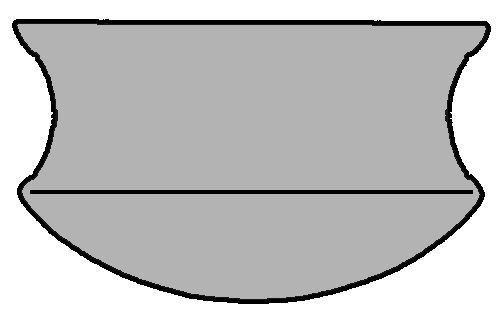
\includegraphics[width=.1\textwidth]{fig/Abb_GefFormen/G1a2_NGO87-102-27.png} & 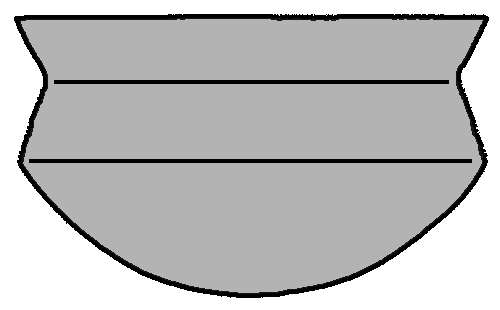
\includegraphics[width=.1\textwidth]{fig/Abb_GefFormen/G2e_INS87-102-2.png} & 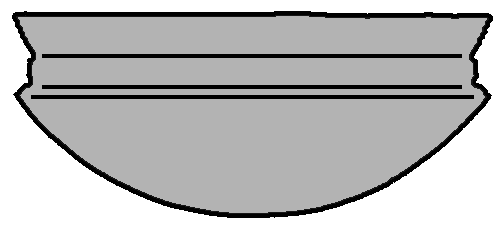
\includegraphics[width=.1\textwidth]{fig/Abb_GefFormen/G2a_NGO87-102-21.png} & 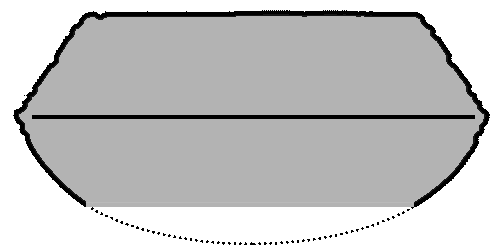
\includegraphics[width=.1\textwidth]{fig/Abb_GefFormen/G2h_MND85-101-33etc.png} & Gefäße mit abknickender Wandung & \\[.11\textwidth]
 & \textbf{G} & 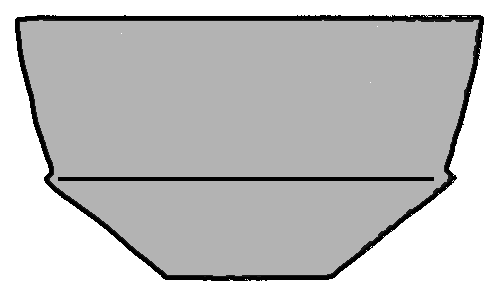
\includegraphics[width=.1\textwidth]{fig/Abb_GefFormen/G2b_ITN87-103-9.png} & 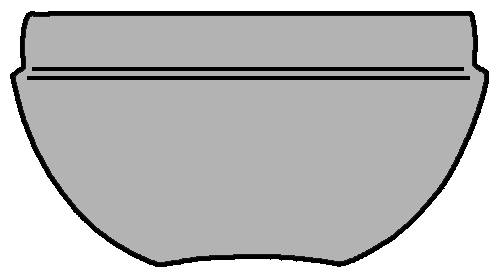
\includegraphics[width=.1\textwidth]{fig/Abb_GefFormen/G2c_MSG87-102-11.png} & 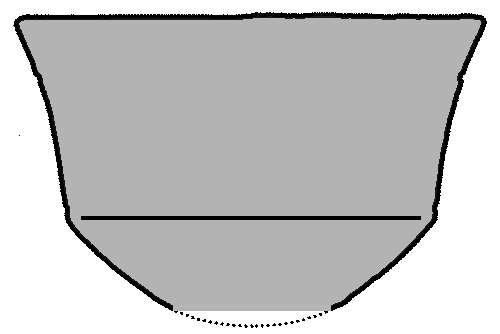
\includegraphics[width=.1\textwidth]{fig/Abb_GefFormen/G2f_MSG87-101-49.png} & 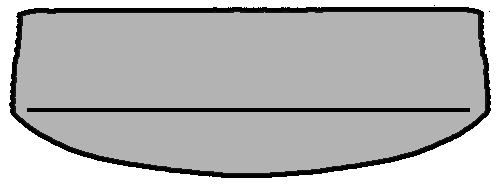
\includegraphics[width=.1\textwidth]{fig/Abb_GefFormen/G2g_GE2_BLK87-1-1-3-1-2.png} & 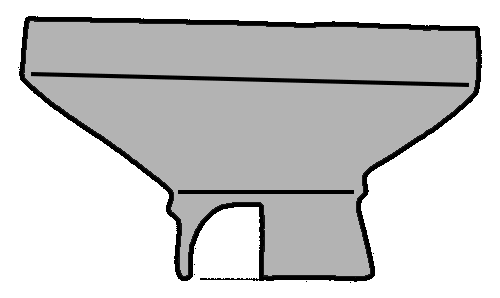
\includegraphics[width=.1\textwidth]{fig/Abb_GefFormen/G2g_MUN87-1-0-2-3-1.png} & 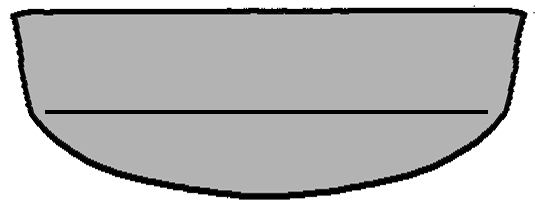
\includegraphics[width=.1\textwidth]{fig/Abb_GefFormen/G8c_Coart1907_TafXII175_neu.png} &  & Schalenförmige Gefäße mit abknickender Wandung & \\[.11\textwidth]
 & \textbf{H} & 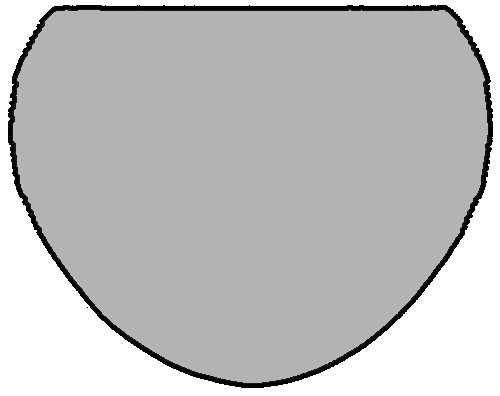
\includegraphics[width=.1\textwidth]{fig/Abb_GefFormen/G8e_kpt85-101-10.png} & 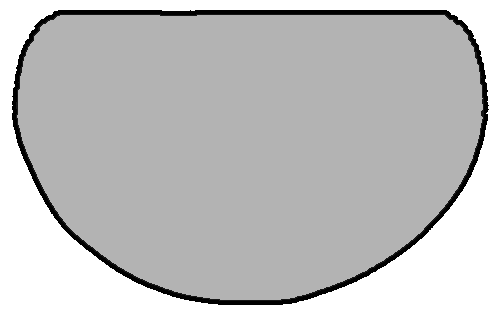
\includegraphics[width=.1\textwidth]{fig/Abb_GefFormen/G8d_MBN85-501-1.png} &  &  &  &  &  & Schalenförmige Gefäße mit konvexer Wandung und einbiegendem Rand & \\[.11\textwidth]
 & \textbf{I} & 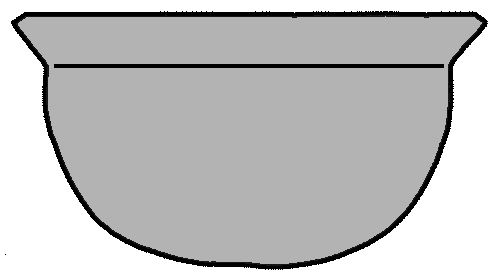
\includegraphics[width=.1\textwidth]{fig/Abb_GefFormen/G8b_BYN87-101-9.png} & 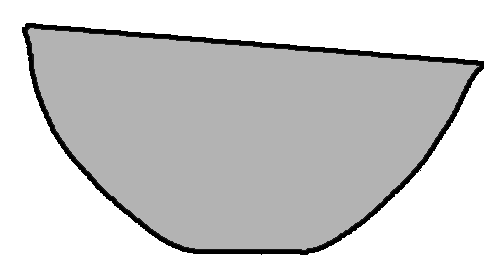
\includegraphics[width=.1\textwidth]{fig/Abb_GefFormen/G9a_DON85-102-120.png} & 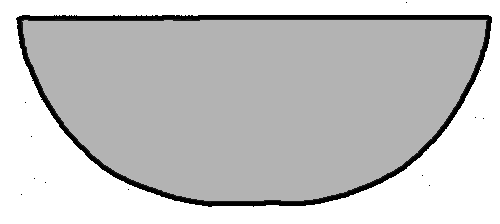
\includegraphics[width=.1\textwidth]{fig/Abb_GefFormen/G8a_BTW87-101-43.png} & 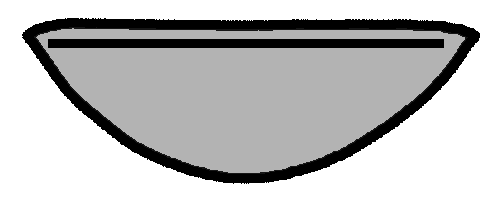
\includegraphics[width=.05\textwidth]{fig/Abb_GefFormen/G8a2_ngk01_PDM87-101-105.png} &  &  &  & Schalenförmige Gefäße mit konvexer Wandung & \\[.11\textwidth]
 & \textbf{J} & 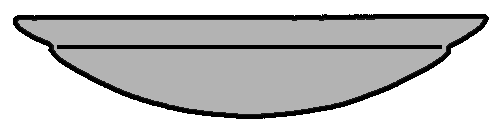
\includegraphics[width=.1\textwidth]{fig/Abb_GefFormen/G12a_NGO87-102-30.png} &  &  &  &  &  &  & Tellerförmige Gefäße & \\[.11\textwidth]
%\bottomrule
\end{sftabular}
}}
	\caption{Keramik: Gefäßtypen (G6 nach \cite[Taf.~XII.175]{Coart.1907}).}
	\label{tab:Keramik_GefFormen}
\end{figure*}

\begin{figure*}[p]
	\centering
	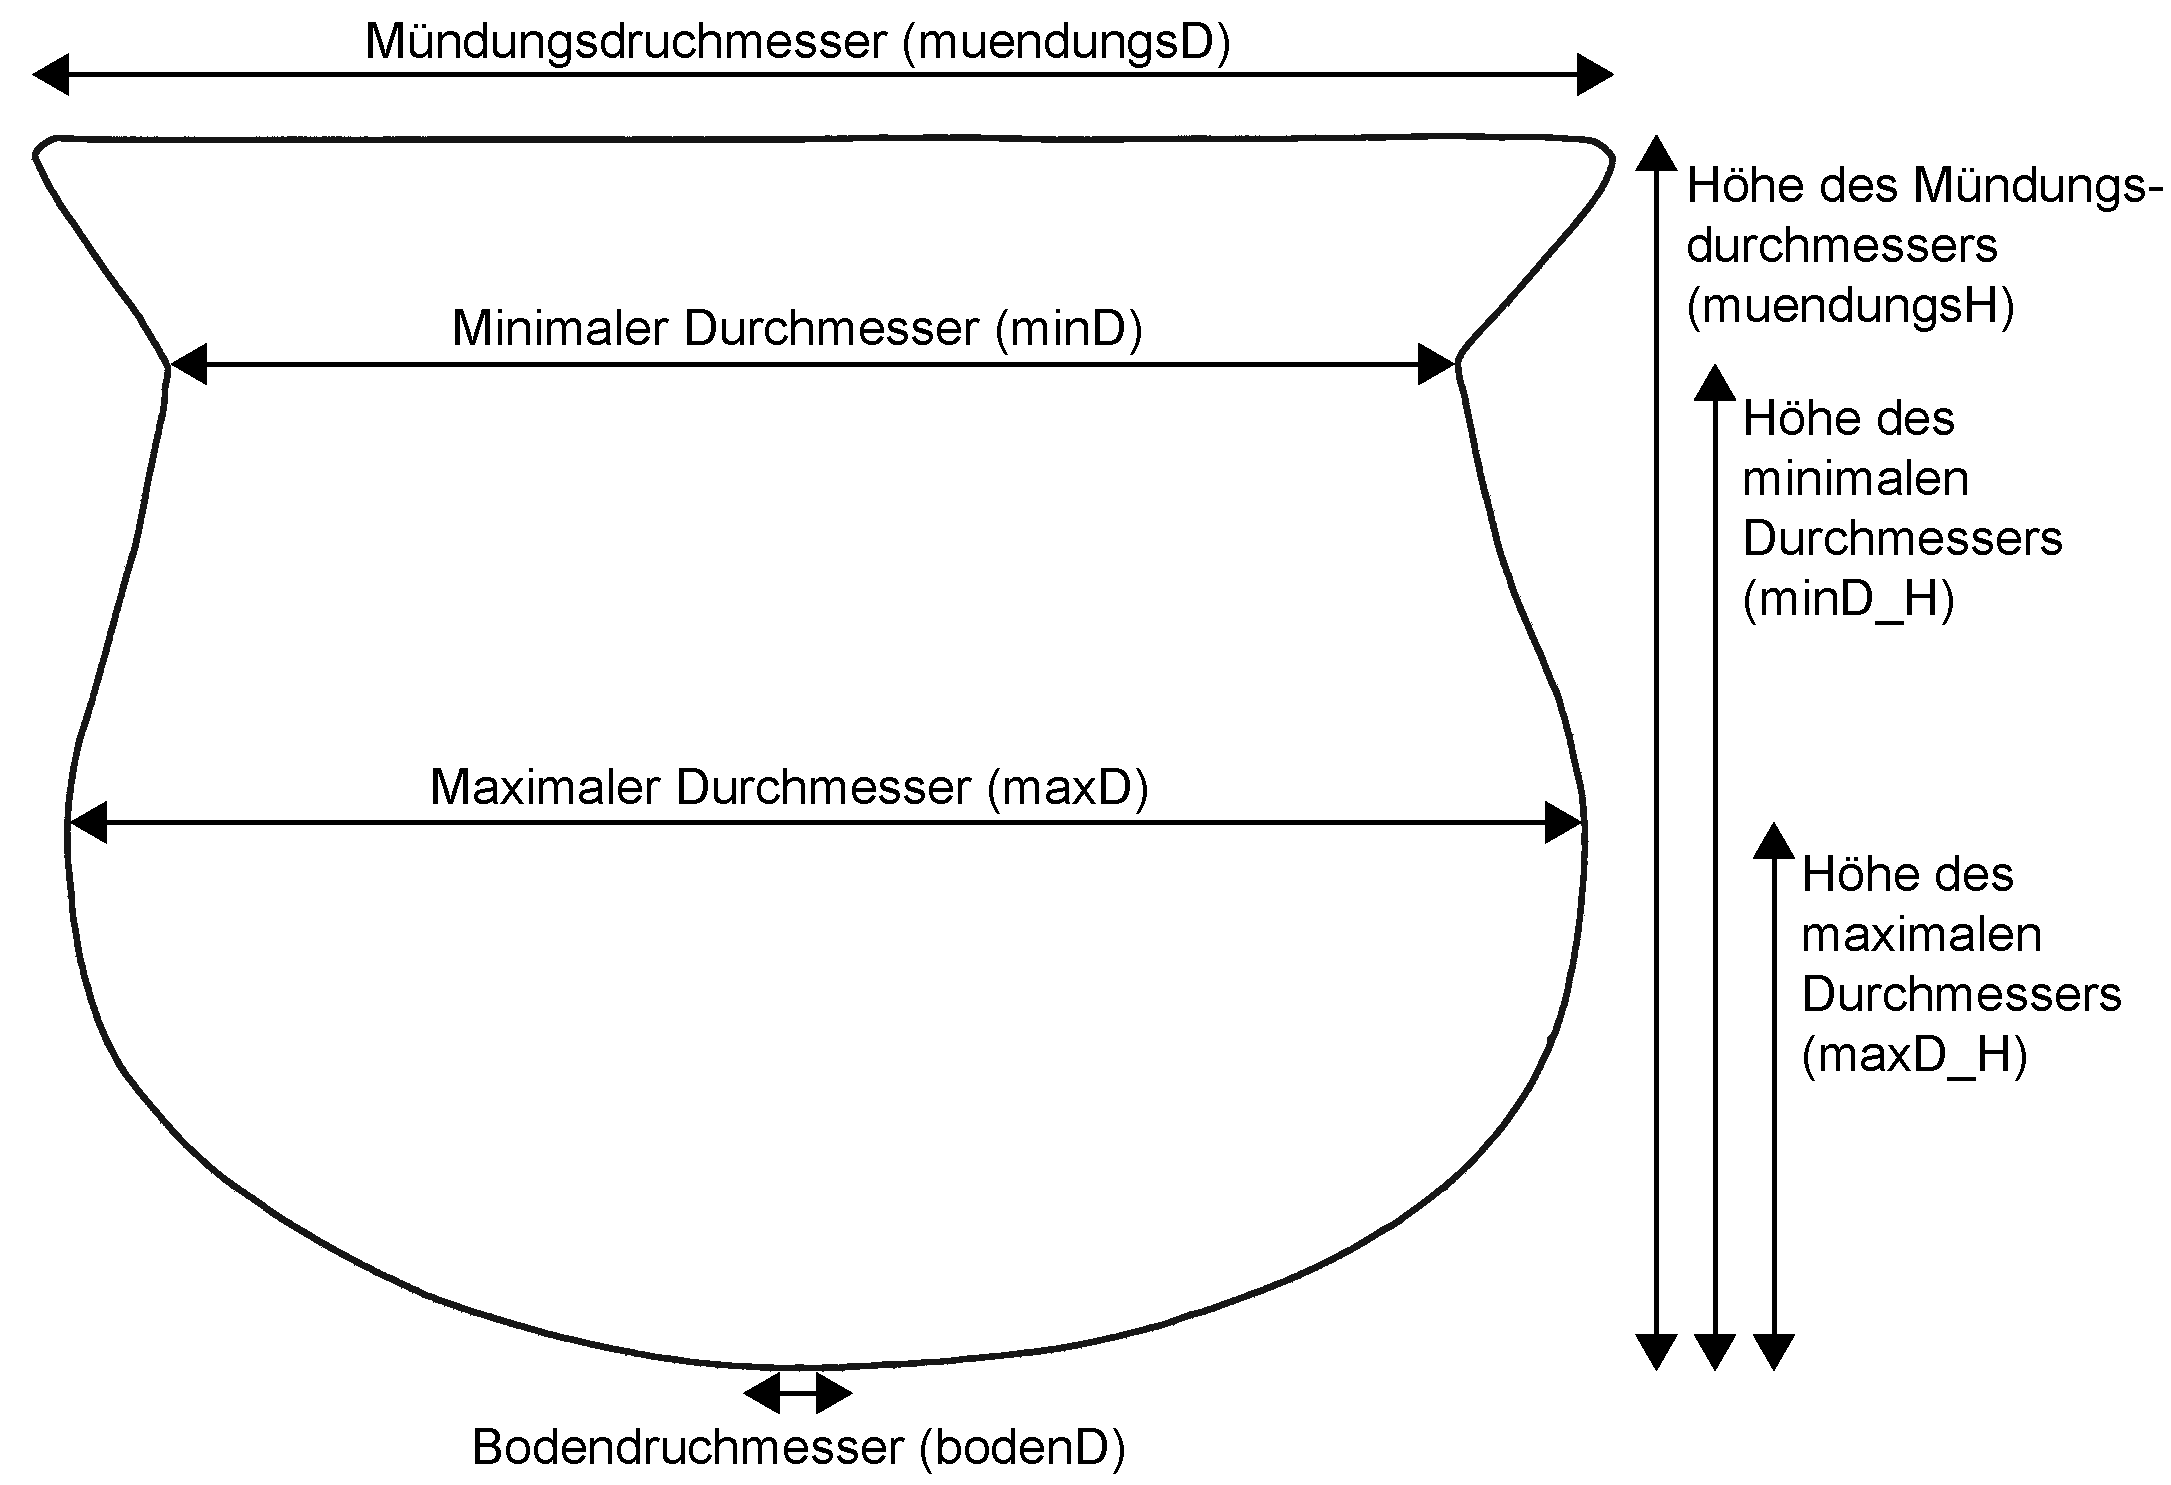
\includegraphics[width=.66\textwidth]{misc/Systematik/GefaesseAbmessungenSystematik.pdf}
	\caption{Keramik: Aufnahmeschema für die Gefäßabmessungen \parencite[nach][siehe Abb.~\ref{fig:DB-Schema} für die Attributnamen]{Wicke.2011}.}
	\label{fig:GefAbmessungen_Schema}
\end{figure*}

\begin{figure*}[p]
	\centering
	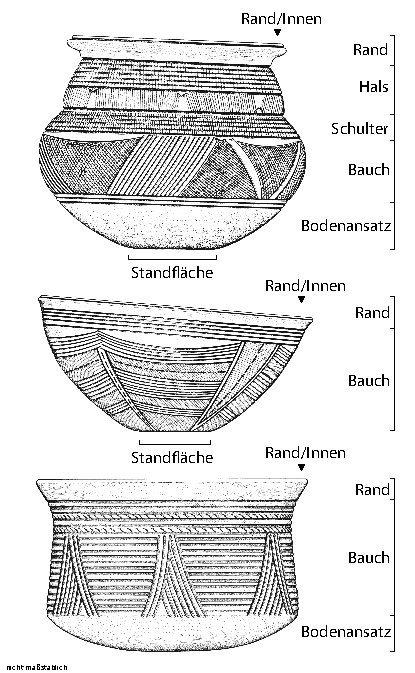
\includegraphics[width=.5\textwidth]{misc/Systematik/Keramik_Systematik_Verzierungszonen.pdf}
	\caption{Keramik: Gefäßzonen-Systematik die für die Beschreibung morphologischer Ausprägungen sowie Verzierungen herangezogen wurden.}
	\label{fig:Keramik_VerzZonen}
\end{figure*}

\paragraph{Gefäßform}
$\;$ \\
Im Rahmen der Auswertung der Gefäßkeramik konnten zehn verschiedene Grundformen unterschieden werden (Tab.~\ref{tab:Keramik_GefFormen} A--J). Diese ließen sich weiter in Varianten (Tab.~\ref{tab:Keramik_GefFormen} 1--7) differenzieren, wodurch sich 41 Gefäßtypen ableiten ließen. Die gewählte Systematisierung der beobachteten Formen war für die angestrebte diachrone Untersuchung unerlässlich, da sich Gefäßformen einerseits zwar im Zeit-Raum-Kontinuum verändern, andererseits sich die Grundformen aber auch immer wiederholen \parencite[86]{Saev.2015}. Die von \textcite{Wotzka.1995} genutzte Systematisierung, die keine Grundformen kennt und zusammengenommen 115 Gefäßformen umfasst, konnte aufgrund ihrer spezifisch auf das Material aus dem Inneren Kongobecken zugeschnittenen Ausprägung nicht übernommen werden.

Insgesamt war bei 2178 Gefäßeinheiten (GE; 41\,\%) eine Ansprache der Gefäßform möglich. Die Proportionen der GE wurden, wo das Abnehmen der entsprechenden Maße möglich war, unter Einsatz von sieben Messstrecken systematisch erfasst (Abb.~\ref{fig:GefAbmessungen_Schema}).\footnote{Im Laufe der Materialaufnahme erwies es sich als problematisch, dass das verwendete Aufnahmeschema für die Höhenwerte von der Standfläche eines Gefäßes ausgeht. Bei einer hohen Zahl von GE fehlte der untere Gefäßteil. Die Höhen der Mündung und minimaler sowie maximaler Durchmesser ließen sich so nicht aufnehmen. Da das Problem erst spät in der Aufnahme zu Tage trat, wurde von einer systematischen Anpassung der Vermessung abgesehen. In Fällen, in den eine Bestimmung der fehlenden Partie in akzeptabler Weise möglich schien, wurde die hypothetische Position der Standfläche rekonstruiert und protokolliert.} Die Abmessungen wurden mit einer Messgenauigkeit von 0,5\,cm aufgenommen, wodurch die Proportionen der von Hand aufgebaute Keramik des Arbeitsgebiet angemessen repräsentiert sind.\footnote{Der Unterschied zwischen Mündungsweite, der tatsächlichen Gefäßöffnung und dem Randdurchmesser wurde nicht ausdifferenziert \parencite[siehe][88]{Saev.2015}.}

Die morphologischen Ausprägungen einzelner GE, wie auch das Dekor (siehe Kap.~\ref{sec:AufnahmeVerzierungen}), wurden nach vordefinierten Gefäßzonen aufgegliedert aufgenommen (Abb.~\ref{fig:Keramik_VerzZonen}). Die Abgrenzung der einzelnen Zonen wurde auf Basis markanter Wendepunkten am Profilverlauf der GE vorgenommen.

\paragraph{Randform}\label{sec:Randform}
$\;$ \\
Die Aufnahme der Ränder erfolgte gemäß einer Systematik, die sich in ersten Linie an der grundsätzlichen Ausrichtung des Randes orientiert. Differenziert wurden parallele, ausbiegende sowie einbiegende Ränder (Tab.~\ref{tab:Keramik_RandFormen}: A--C). Innerhalb dieser Grundtypen wurden mehrere charakteristische Varianten unterschieden. Parallele Ränder können neben der einfache Grundform auch als umgelenkte, T-förmige sowie verdickte Formen vorkommen (Tab.~\ref{tab:Keramik_RandFormen}: A2--A4). Die aus- wie die einbiegenden Ränder wurden noch in konkave sowie konvexe Varianten unterschieden (Tab.~\ref{tab:Keramik_RandFormen}: B2--B3, C2--C3):

\vspace{1em}
%\setlength\LTleft{0pt}
\begin{tabular}{@{}ll@{}}
A1 & parallel \\
A2 & umgelegt \\
A3 & T-förmig \\
A4 & verdickt \\
B1 & ausbiegend \\
B2 & konkav ausbiegend \\
B3 & konvex ausbiegend \\
C1 & einbiegend \\
C2 & konkav einbiegend \\
C3 & konvex einbiegend \\
\end{tabular}
\addtocounter{table}{-1}
\vspace{1em}

\noindent An die Grundform angefügten Parameter \enquote*{.1} sowie \enquote*{.2} zeigen \enquote*{kurze} beziehungsweise \enquote*{lange} Varianten der entsprechenden Randform an. Spezifischere und diagnostische Variationen der Grundformen wurden im weiteren Verlauf der Aufnahme durch Hinzusetzen individueller Zählnummern, beginnend ab dem Schlüssel-Zusatz \enquote*{.3}, angefügt. Insgesamt ergaben sich 10 Grundformen der Randgestaltung (Tab.~\ref{tab:Keramik_RandFormen}) sowie 26 unterscheidbare Variationen.\footnote{Wie bereits bei den Gefäßformen (Kap.~\ref{tab:Keramik_GefFormen}) reflektiert die gewählte Form der Systematisierung das Bestreben, die Aufnahme des Untersuchungsmaterials vor dem Hintergrund der dieser Arbeit zugrundeliegenden diachronen Fragestellungen durchzuführen.}

\begin{figure*}[!tb]
	\centering
	{\small
		\begin{tabular}{ >{\centering\arraybackslash} m{.025\textwidth} >{\centering\arraybackslash} m{.1\textwidth} >{\centering\arraybackslash} m{.1\textwidth} >{\centering\arraybackslash} m{.1\textwidth} >{\centering\arraybackslash} m{.1\textwidth}}
			%\toprule
			& \textbf{1} & \textbf{2} & \textbf{3} & \textbf{4} \\
			%\midrule
			\textbf{A} & 
\includegraphics[height=.1\textwidth]{misc/Systematik/3_Rand/A1.pdf} & 
\includegraphics[height=.1\textwidth]{misc/Systematik/3_Rand/A2.pdf} & 
\includegraphics[height=.1\textwidth]{misc/Systematik/3_Rand/A3.pdf} & \includegraphics[height=.1\textwidth]{misc/Systematik/3_Rand/A4.pdf} \\
			\textbf{B} & \includegraphics[height=.1\textwidth]{misc/Systematik/3_Rand/B1.pdf} & \includegraphics[height=.1\textwidth]{misc/Systematik/3_Rand/B2.pdf} & \includegraphics[height=.1\textwidth]{misc/Systematik/3_Rand/B3.pdf} & \\
			\textbf{C} & \includegraphics[height=.1\textwidth]{misc/Systematik/3_Rand/C1.pdf} & \includegraphics[height=.1\textwidth]{misc/Systematik/3_Rand/C2.pdf} & \includegraphics[height=.1\textwidth]{misc/Systematik/3_Rand/C3.pdf} & \\
			%\bottomrule
	\end{tabular}}
	\caption{Keramik: Systematisierung der grundsätzlichen Randformen (A--C).}
	\label{tab:Keramik_RandFormen}
\end{figure*}

Die häufigste Randform, einfach ausbiegende Ränder (\enquote*{B1}), macht 24,8\,\% aller bestimmten Randformen aus, gefolgt von konkav ausbiegenden Rändern (\enquote*{B2}), die in 13,3\,\% aller Fälle beobachtet wurden. Die kurze Variante gerade ausbiegender Rändern (\enquote*{B1.1}) macht 11,7\,\% aus, während parallel, gerade aufsteigende Ränder (\enquote*{A1}) auf einen Anteil von 10\,\% kommen. Alle übrigen Varianten liegen jeweils im Bereich von unter 7\,\% der beobachteten Ränder. Zusammengenommen repräsentiere diese, einzeln nur wenig vertretenen Formen, 40\,\% der aufgenommen Gefäßränder. Werden die unterschiedenen Variationen den jeweiligen Grundformen (Tab.~\ref{tab:Keramik_RandFormen}) zugerechnet, so machen einfach ausbiegende Ränder (\enquote*{B1}) 42,4\,\% aller bestimmten Randformen aus. Weiter generalisierend sind insgesamt 68,5\,\% aller Rändern ausbiegend (\enquote*{B}), während 25\,\% parallel (\enquote*{A}) verlaufen und nur 6,5\,\% einbiegend (\enquote*{C}) sind.

\begin{table*}[!tb]
	\centering
	{\small
		\begin{tabular}{@{}m{.1\textwidth}m{.1\textwidth}m{.4\textwidth}@{}}
			\toprule
			& \textbf{Typ} & \textbf{Beschreibung} \\
			\midrule
			\includegraphics[height=.05\textwidth]{misc/Systematik/2_Mdg/M1_ATANGANA1988OkoloS162_1.png} & M1 & rund \\
			\includegraphics[height=.05\textwidth]{misc/Systematik/2_Mdg/M2_ATANGANA1988OkoloS162_2.png} & M2 & spitz \\
			\includegraphics[height=.05\textwidth]{misc/Systematik/2_Mdg/M3_ATANGANA1988OkoloS162_3.png} & M3 & gerade/flach/horizontal abgestrichen \\
			\includegraphics[height=.05\textwidth]{misc/Systematik/2_Mdg/M4_ATANGANA1988OkoloS162_4.png} & M4 & gerillt \\
			\includegraphics[height=.05\textwidth]{misc/Systematik/2_Mdg/M5_schraegAussen.png} & M5 & schräg nach außen abgestrichen \\
			\includegraphics[height=.05\textwidth]{misc/Systematik/2_Mdg/M6_schraegInnen.png} & M6 & schräg nach innen abgestrichen \\
			\bottomrule
	\end{tabular} }
	\caption{Keramik: Randlippe \parencite[erweitert nach][162f Tab.~24]{Atangana.1988}.}
	\label{tab:MdgFormen}
\end{table*}

\clearpage\paragraph{Randlippe}
$\;$ \\
Die Ausprägung der Randlippe, in diesem Zusammenhang auch \enquote*{Gefäßmündung} genannt, wurde in Anlehnung an die von \textcite[162f Tab.~24]{Atangana.1988} genutzte Systematik losgelöst von der Randform aufgenommen (Tab.~\ref{tab:MdgFormen}).\footnote{\textcite[48]{Wotzka.1995} erfasste die Ausprägung der Randlippe nicht separat; sie bildete vielmehr eine mögliche Variation des \enquote*{Randtyps} ab. Ähnlich ging auch \textcite[110]{Jesse.2003} vor.} Die Einteilung Atanganas wurde dabei um die beiden Formen \enquote*{M5} sowie \enquote*{M6}, die schräg nach außen oder innen abgestrichene Randlippen repräsentieren, erweitert. Die Varianten \enquote*{M1} bis \enquote*{M5} sind jeweils in Häufigkeiten zwischen 13,5 bis 26,4\,\% vertreten, lediglich schräg nach innen abgestrichene Randlippen (\enquote*{M6}) kommen mit nur 3,9\,\% deutlich seltener vor.

\begin{figure*}[!tb]
	\centering
	\includegraphics[width=\textwidth]{misc/Systematik/10_Boden/Wotzka1995_440Taf6_modDS.jpg}
	\caption{Keramik: Bodenformen \parencite[nach][440 Taf.~6]{Wotzka.1995}.}
	\label{fig:Keramik_BodenFormen}
\end{figure*}

\paragraph{Bodenform}\label{sec:Bodenform}
$\;$ \\
Die Unterscheidung der Ausformung des Bodens gründete sich auf die von \textcite[440 Taf.~6]{Wotzka.1995} aufgestellten Systematik, die um eine Form \enquote*{B15} erweitert wurde. Die neue Bodenform \enquote*{B15} beschreibt Gefäße, die auf einzelnen \enquote*{Füßchen} stehen. Im untersuchten Material fanden sich lediglich zwei GE mit drei symmetrisch am Unterteil eines ansonsten rund ausgeformten Bodens \enquote*{Füßchen} (Taf.~1.2, 2.1). Im Detail wurden folgende Bodenformen unterschieden (Abb.~\ref{fig:Keramik_BodenFormen}.):
\setlength\LTleft{0pt}
\begin{longtable}{@{}ll@{}}
	B1 & Rundboden \\
	B2 & Linsenboden \\
	B3 & Spitzboden \\
	B4 & einfacher Flachboden \\
	B5 & innen aufgewölbter Flachboden  \\
	B6 & Flachboden mit konkaver Standfläche \\
	B7 & Omphalosboden \\
	B8 & Riefenprofilierter Flachboden \\
	B9 & Profiliert abgesetzter Flachboden \\
	B10 & Riefenabgesetzter Flachboden \\
	B11 & abgesetzter Flachboden \\
	B12 & Flachboden mit deutlich einziehender Unterseite \\
	B13 & Standring / Hohlfuß \\
	B14 & massiver Standfussboden \\
	B15 & Boden mit abgesetzten Standfüßen \\
\end{longtable}
\addtocounter{table}{-1}

\noindent Insgesamt konnte die Bodenform lediglich bei 6\,\% aller GE angesprochen werden. Dieser geringe Anteil liegt zu einen gewissen Grad an den Schwierigkeiten, die mit der Ansprache runder Böden (\enquote*{B1}) verbunden sind, die leicht für Fragmente der Gefäßwandung fehlinterpretiert werden können. Zusammengenommen machen runde Böden (\enquote*{B1}) aber knapp 49\,\% aller bestimmten Böden aus. Einfache Flachböden (\enquote*{B4}) kommen mit 24\,\% am zweithäufigsten vor. Gefolgt werden sie von Linsenböden (\enquote*{B2}) mit 6\,\%, Standringböden mit Hohlfuß (\enquote*{B13}) mit ebenfalls 6\,\% sowie Flachböden mit konkaver Standfläche (\enquote*{B6}) mit 5\,\%. Die übrigen Formen kommen lediglich als Einzelfunde beziehungsweise bei weniger als zehn GE vor. Der von \textsc{Wotzka} (ebd. 440 Taf.~6) beschrieben Typ \enquote*{B14} wurde nicht beobachtet.


\subsubsection{Verzierung}\label{sec:AufnahmeVerzierungen}

Die Verzierungen der Keramik wurden für jede Gefäßeinheit (GE) individuell und mit Bedacht auf die Gefäßregion aufgenommen (siehe Abb.~\ref{fig:Keramik_VerzZonen}).\footnote{Während formale Ansprachen wie die Gefäßform in einer 1:n-Beziehung in einer Datenbank abgebildet werden können, eine GE kann lediglich eine Gefäßform oder Randform aufweisen, können verschiedene Verzierungen auf verschiedenen Gefäßbereichen unterschiedlich häufig vorkommen. Die vorliegende Kardinalität der Entitätstypen \enquote*{Objekt}, \enquote*{Gefäßposition} und \enquote*{Verzierungselement} können in dem genutzten relativen Datenbankschema nicht direkt abgebildet werden. Die Entitäten jeder dieser Entitätstypen können mit beliebig vielen Entitäten der anderen beiden Entitätstypen in Beziehung stehen. Konkret ist hiermit gemeint, dass eine GE an mehreren Stellen mit mehreren Verzierungselementen dekoriert sein kann. Als Lösung wird eine Konkordanztabelle genutzt, welche die Primärschlüssel der genannten Entitätstypen als Fremdschlüssel-Paare beinhaltet. Die Beziehungen der drei Entitätstypen werden im Datenmodell durch drei getrennten 1:n-Beziehungen aufgelöst (Abb.~\ref{fig:DB-Schema}).} Basierend auf der Kombination aus Verzierungstechnik und -motiv wurden Verzierungselemente erarbeitet (Tab.~\ref{tab:Verzierungselemente}; Abb.~\ref{fig:Keramik_VerzSystematik}).\footnote{Die Klassifizierung der einzelnen Verzierungselemente lehnt sich dabei stark an \textcite{Wotzka.1995} an, beinhaltete aber auch lose Bezüge zu Systematiken für die Bandkeramik \parencites{Stehli.1973}{Stehli.1977}{Kneipp.1998} und das südfranzösische Frühneolithikum \parencites[126f. Abb.~3]{Manen.2002}[auch bei][]{Linstadter.2013}.} Diese bilden in der Aufnahme der Verzierungen wie deren Auswertung die analytische Grundeinheit.

\begin{figure*}[p]
 \centering
 \includegraphics[width=.85\textwidth]{misc/Systematik/VerzierungenSystematik.pdf}
 \caption{Keramik: Verzierungstechniken, Verzierungswerkzeuge und Verzierungselemente.}
 \label{fig:Keramik_VerzSystematik}
\end{figure*}

\afterpage{%
\clearpage
{\small \begin{table*}[p]

\begin{multicols}{2}
\noindent
{\scriptsize\begin{sftabular}{@{}m{.05\columnwidth} m{.1\textwidth} m{.63\columnwidth}@{}}
\toprule
\multicolumn{2}{@{}l@{}}{\textbf{Schlüssel}} &  \textbf{Kurzbeschreibung} \\
\midrule
01.1 & \includegraphics[width=.1\textwidth]{tbl/Tab_VerzElemente/V03a_PIK87-1-7-1.png} & \textit{Schachbrett}-Muster aus horizontalen und vertikalen Ritzlinien \\
01.2 & \includegraphics[width=.1\textwidth]{tbl/Tab_VerzElemente/V03b_PIK87-1-6-16.png} & \textit{Schachbrett}-Muster aus diagonalen Ritzlinien \\
01.3 & \includegraphics[width=.1\textwidth]{tbl/Tab_VerzElemente/V03c_PIK87-1-8-6.png} & \textit{Schachbrett}-Muster aus horizontalen und diagonalen Ritzlinien \\
01.4 & \includegraphics[width=.1\textwidth]{tbl/Tab_VerzElemente/V03d_PIK87-1-9-7.png} & \textit{Schachbrett}-Muster aus diagonalen und vertikalen Ritzlinien \\
01.5 & \includegraphics[width=.1\textwidth]{tbl/Tab_VerzElemente/V01b_PIK87-1-5-7.png} & Wellenlinien \\
01.6 & \includegraphics[width=.1\textwidth]{tbl/Tab_VerzElemente/V12a1_MSG87-102-8.png} & Zickzack-Linien \\
01.7 & \includegraphics[width=.1\textwidth]{tbl/Tab_VerzElemente/V12c_Gef9_CAM07-3-1-278-306.png} & Rillen in Fischgrät-Muster \\
01.8 & \includegraphics[width=.1\textwidth]{tbl/Tab_VerzElemente/V04d_PIK87-101-43-46.png} \includegraphics[width=.1\textwidth]{tbl/Tab_VerzElemente/V04e_NGO87-102-28-29.png} & Rillen gefüllte Flächen (Dreiecke, Rauten u.~a.) \\
01.9 & \includegraphics[width=.1\textwidth]{tbl/Tab_VerzElemente/V10a_PIK87-101-51.png} & feine vertikale oder horizontale Rillen \\
01.10 & \includegraphics[width=.1\textwidth]{tbl/Tab_VerzElemente/V10b_PIK87-101-40.png} & feine diagonale Rillen \\
01.11 & \includegraphics[width=.1\textwidth]{tbl/Tab_VerzElemente/V11b1_LKW87-186-1-2-5.png} & Muster aus überkreuzten Rillen \\
02.1 & \includegraphics[width=.1\textwidth]{tbl/Tab_VerzElemente/V01a_PIK87-1-8-6.png} & horizontale Riefen \parencite[siehe Muster \enquote{ISpeg5} von][251 Abb. 30.5 ]{GouemGouem.20102011} \\
02.2 & \includegraphics[width=.1\textwidth]{tbl/Tab_VerzElemente/V01c_PIK87-1-8-6.png} & vertikale Riefen \\
\bottomrule
\end{sftabular}}

\noindent
{\scriptsize\begin{sftabular}{@{}m{.05\columnwidth} m{.1\textwidth} m{.63\columnwidth}@{}}
\toprule
\multicolumn{2}{@{}l@{}}{\textbf{Schlüssel}} &  \textbf{Kurzbeschreibung} \\
\midrule
02.3 & \includegraphics[width=.1\textwidth]{tbl/Tab_VerzElemente/V01e_PIK87-1-8-6.png} & diagonale Riefen \\
02.4 & \includegraphics[width=.1\textwidth]{tbl/Tab_VerzElemente/V01e2_MLB85-1-3-2-5-35.png} & horizontales Band aus kurzen diagonalen Riefen \\
02.5 & \includegraphics[width=.1\textwidth]{tbl/Tab_VerzElemente/V01d_PIK87-101-7.png} & gebogene Riefen \\
02.6 & \includegraphics[width=.1\textwidth]{tbl/Tab_VerzElemente/V01f_MUN87-2-1-1-5-2.png} & spitz zusammenlaufende gebogene Riefen \\
02.7 & \includegraphics[width=.1\textwidth]{tbl/Tab_VerzElemente/V04c_PIK87-1-3-9.png} & sehr breite Riefen (\textgreater\,5\,mm) \\
03.1 & \includegraphics[width=.1\textwidth]{tbl/Tab_VerzElemente/V06e.png} & große Eindrücke, Fingereindrücke \\
04.1 & \includegraphics[width=.1\textwidth]{tbl/Tab_VerzElemente/V02a_PIK87-1-8-6.png} & Wiegeband mit Kamm \\
04.2 & \includegraphics[width=.1\textwidth]{tbl/Tab_VerzElemente/V02b_MUN87-2-1-1-4-2.png} & Wiegeband (siehe Muster \enquote{IIIPla1z} von \textsc{Gouem Gouem} 2010/2011: 117 Abb. 9.3.a ) \\
04.3 & \includegraphics[width=.1\textwidth]{tbl/Tab_VerzElemente/V05e_INS87-102-2.png} & gruppierte Eindrücke \\
04.4 & \includegraphics[width=.1\textwidth]{tbl/Tab_VerzElemente/V05f_SSL87-101-143.png} & gegenständige Eindrücke \\
04.5 & \includegraphics[width=.1\textwidth]{tbl/Tab_VerzElemente/V05j_SSL87-101-5.png} & kleine Flächen aus gegenständigen, halbrunden Eindrücken \\
04.6 & \includegraphics[width=.1\textwidth]{tbl/Tab_VerzElemente/V05h_DON85-102-a.png} & flache, winkelige Eindrücke \\
04.7 & \includegraphics[width=.1\textwidth]{tbl/Tab_VerzElemente/V05i1_MLB85-1-2-3.png} & kleine Kreisaugen-Eindrücke \\
& & \\[1mm]
\bottomrule
\end{sftabular}}
\end{multicols}
\caption{Keramik: Verzierungselemente. Für die ersten beiden Stellen der Schlüsselzahl -- die  Verzierungstechnik -- siehe \textsc{Wotzka} (1995: 44 Tab.~3).}
\label{tab:Verzierungselemente}
\end{table*}

\addtocounter{table}{-1}
\begin{table*}[p]
\begin{multicols}{2}
\noindent
{\scriptsize\begin{sftabular}{@{}m{.05\columnwidth} m{.1\textwidth} m{.63\columnwidth}@{}}
\toprule
\multicolumn{2}{@{}l@{}}{\textbf{Schlüssel}} &  \textbf{Kurzbeschreibung} \\
\midrule
04.8 & \includegraphics[width=.1\textwidth]{tbl/Tab_VerzElemente/V09l_MKA87-102-1.png} & dreieckige Eindrücke/Dreieckstempel \\
04.9 & \includegraphics[width=.1\textwidth]{tbl/Tab_VerzElemente/V09j_MIS87-101-56.png} & flächig angeordnete, horizontale Bänder kleiner Eindrücke \\
04.10 & \includegraphics[width=.1\textwidth]{tbl/Tab_VerzElemente/V09k_MIS87-101-56.png} & lose flächig verteilte kleine Eindrücke \\
04.11 & \includegraphics[width=.1\textwidth]{tbl/Tab_VerzElemente/V09i2_MKL85-101-114.png} & runde bis leicht ovale Eindrücke \\
04.12 & \includegraphics[width=.1\textwidth]{tbl/Tab_VerzElemente/V09a1_PIK87-1-14-1.png} & diagonale Eindrücke \\
04.13 & \includegraphics[width=.1\textwidth]{tbl/Tab_VerzElemente/V09n_SSL87-101-19.png} & leicht gewellte Bänder aus diagonalen oder vertikalen Eindrücken \\
04.14 & \includegraphics[width=.1\textwidth]{tbl/Tab_VerzElemente/V09a2_DON85-102-120.png} & horizontales oder vertikales Band aus linearen Eindrücken \\
04.15 & \includegraphics[width=.1\textwidth]{tbl/Tab_VerzElemente/V09b_PIK87-1-8-10.png} & vertikale Eindrücke \\
04.16 & \includegraphics[width=.1\textwidth]{tbl/Tab_VerzElemente/V09c1_PIK87-1-13-1.png} \includegraphics[width=.1\textwidth]{tbl/Tab_VerzElemente/V09c2_DON85-102-117.png} & Eindrücke in Rillen (siehe Muster \enquote{ISpeg5/ISpeg11} bei \textsc{Gouem Gouem} 2010/2011251, 251 Abb. 30.5) \\
04.17 & \includegraphics[width=.1\textwidth]{tbl/Tab_VerzElemente/V12b_INS87-102-2.png} & gegenständige Dreiecke in horizontalem Band \\
04.18 & \includegraphics[width=.1\textwidth]{tbl/Tab_VerzElemente/V11b2_DON85-102-126.png} & Bänder aus x-förmigen Eindrücken \\
04.19 & \includegraphics[width=.1\textwidth]{tbl/Tab_VerzElemente/V09h1_PDM87-101-12.png} & lange gebogene Eindrücke in Reihen \\
04.20 & \includegraphics[width=.1\textwidth]{tbl/Tab_VerzElemente/V09h2_MIT87-102-19.png} & kurze gebogene Eindrücke (Fingernagel) \\
04.21 & \includegraphics[width=.1\textwidth]{tbl/Tab_VerzElemente/V05i3_MBA11-1-1_DSC_0507_b.png} & Eindrücke mit Kaurischnecken oder Imitation \\
& & \\
\bottomrule
\end{sftabular}}

\noindent
{\scriptsize\begin{sftabular}{@{}m{.05\columnwidth} m{.1\textwidth} m{.63\columnwidth}@{}}
\toprule
\multicolumn{2}{@{}l@{}}{\textbf{Schlüssel}} &  \textbf{Kurzbeschreibung} \\
\midrule
05.1 & \includegraphics[width=.1\textwidth]{tbl/Tab_VerzElemente/V02c_PDM87-101-125.png} & diagonaler Kammeindruck \\
05.2 & \includegraphics[width=.1\textwidth]{tbl/Tab_VerzElemente/V12a3_MKL85-101-105.png} & Band aus zickzackartig angeordneten Kammeindrücken \\
05.3 & \includegraphics[width=.1\textwidth]{tbl/Tab_VerzElemente/V05a_PIK87-1-2-5.png} & Kammeindruck-Bänder \\
05.4 & \includegraphics[width=.1\textwidth]{tbl/Tab_VerzElemente/V05b_PIK87-101-8.png} & flächiger Kammeindruck \\
08 & \includegraphics[width=.1\textwidth]{tbl/Tab_VerzElemente/V07_MUN87-1-0-2-3-6.png} & \textit{Bnfwa-nfwa} \parencite[Muster: siehe][109--111]{Wotzka.1995} \\
09.1 & \includegraphics[width=.1\textwidth]{tbl/Tab_VerzElemente/V06a1_PIK87-1-2-5.png} & Knubben \\
09.2 & \includegraphics[width=.1\textwidth]{tbl/Tab_VerzElemente/V06b_PIK87-101-8.png} & Plastische Leiste \\
12 & \includegraphics[width=.1\textwidth]{tbl/Tab_VerzElemente/V14_Wotzka1995_Taf91-4.png} & Mattenabdruck \\
13.1 & \includegraphics[width=.1\textwidth]{tbl/Tab_VerzElemente/V13_Gef3_CAM07-12-II-2.png} & Durchlochung der Gefäßwandung \\
14.1 & \includegraphics[width=.1\textwidth]{tbl/Tab_VerzElemente/VB1_YUM87-103-2.png} & Schwarze bis dunkelgraue Bemalung. Die Bemalung erfolgt ausschließlich in Streifen. Eine flächige Bemalung größerer Abschnitte eines Gefäßes wurde nicht beobachtet. \\
14.2 & \includegraphics[width=.1\textwidth]{tbl/Tab_VerzElemente/Vb2_BBS87-Herdgef_E87-04-4.png} & Rote Bemalung. Die Bemalung erfolgt ausschließlich in Streifen sowie in Riefen. Eine flächige Bemalung größerer Abschnitte eines Gefäßes wurde nicht beobachtet. \\
15.1 & \includegraphics[width=.1\textwidth]{tbl/Tab_VerzElemente/V04a_PIK87-1-3-5.png} & diagonaler Kammstrich \\
15.2 & \includegraphics[width=.1\textwidth]{tbl/Tab_VerzElemente/V04b_PIK87-1-2-225.png} & überkreuzter Kammstrich \\
& & \\[1.5mm]
\bottomrule
\end{sftabular}}
\end{multicols}
\caption{Keramik: Verzierungselemente. Für die ersten beiden Stellen der Schlüsselzahl -- die  Verzierungstechnik -- siehe \textsc{Wotzka} (1995: 44 Tab.~3).}
%\label{tab:Verzierungselemente}
\end{table*}

\addtocounter{table}{-1}
\begin{table*}[!tb]
\begin{multicols}{2}
\noindent
{\scriptsize\begin{sftabular}{@{}m{.05\columnwidth} m{.1\textwidth} m{.63\columnwidth}@{}}
\toprule
\multicolumn{2}{@{}l@{}}{\textbf{Schlüssel}} &  \textbf{Kurzbeschreibung} \\
\midrule
15.3 & \includegraphics[width=.1\textwidth]{tbl/Tab_VerzElemente/V05i2a_PIK87-101-17.png} \includegraphics[width=.1\textwidth]{tbl/Tab_VerzElemente/V05i2b_MTB85-101-12.png} & in Kammstrich-Technik hergestellte konzentrische, teilweise sich überlagernde Kreis-Muster \\
17.1 & \includegraphics[width=.1\textwidth]{tbl/Tab_VerzElemente/V06a2_MLB85-101-18.png} & Ösen \\
17.2 & \includegraphics[width=.1\textwidth]{tbl/Tab_VerzElemente/V06a3_LIB85-101-50.png} & Henkel \\
20.1 & \includegraphics[width=.1\textwidth]{tbl/Tab_VerzElemente/V08m_NGA87-101-22.png} & unklar, möglicherweise Mattenabdruck \\
20.2 & \includegraphics[width=.1\textwidth]{tbl/Tab_VerzElemente/V08n_MBK85-101-11.png} & unklar, möglicherweise Textilabdruck \\
21.1 & \includegraphics[width=.1\textwidth]{tbl/Tab_VerzElemente/V08a_BBL85-101-61.png} & \textit{knotted strip} \parencite[Muster: siehe][191 Abb.~1,C]{LivingstoneSmith.2007} \\
21.2 & \includegraphics[width=.1\textwidth]{tbl/Tab_VerzElemente/V08a1_LivingstoneSmith2007_Fig1A.png} & \textit{twisted string} (Muster: siehe \textsc{Livingstone Smith} 2007: 191 Abb.~1,A) \\
21.3 &  \includegraphics[width=.1\textwidth]{tbl/Tab_VerzElemente/V08a2_LivingstoneSmith2007_Fig1B.png} & \textit{alternate knotted strip} (Muster: ebd. 191 Abb.~1,B) \\
21.4 & \includegraphics[width=.1\textwidth]{tbl/Tab_VerzElemente/V08a3_Mayoretal2005.png} & \textit{Accordion-plaited strip} \parencite[Muster: siehe][36 Abb.~4]{Mayor.2005} \\
21.5 & \includegraphics[width=.1\textwidth]{tbl/Tab_VerzElemente/V08b_KPT85-101-10.png}  & Schnitzroulette, das ein Muster aus gegenläufigen gezähnten Bändern erzeugt \\
& & \\[5mm]
\bottomrule
\end{sftabular}}

\noindent
{\scriptsize\begin{sftabular}{@{}m{.05\columnwidth} m{.1\textwidth} m{.63\columnwidth}@{}}
\toprule
\multicolumn{2}{@{}l@{}}{\textbf{Schlüssel}} &  \textbf{Kurzbeschreibung} \\
\midrule
21.6 & \includegraphics[width=.1\textwidth]{tbl/Tab_VerzElemente/V08c_MTB85-101-94.png} & Schnitzroulette, das ein Muster aus gegenläufigen gezackten Bändern erzeugt \\
21.7 & \includegraphics[width=.1\textwidth]{tbl/Tab_VerzElemente/V08e_ILW85-101-11.png} & Schnitzroulette, das ein rautenförmiges Muster erzeugt, wobei das Zentrum erhaben ist \\
21.8 & \includegraphics[width=.1\textwidth]{tbl/Tab_VerzElemente/V08f_GBA85-101-6.png} & Schnitzroulette wie 21.7 jedoch mit einem erhabenen Zentrum und Grat \\
21.9 & \includegraphics[width=.1\textwidth]{tbl/Tab_VerzElemente/V08g_LIB85-101-28.png} & Schnitzroulette, das ein Muster aus dreieckigen Bändern erzeugt \\
21.10 & \includegraphics[width=.1\textwidth]{tbl/Tab_VerzElemente/V08h_BAT85-101-40.png} & Schnitzroulette wie 21.7 jedoch mit einem eingedrückten Zentrum \\
21.11 & \includegraphics[width=.1\textwidth]{tbl/Tab_VerzElemente/V08i_MBK85-101-15.png} & Schnitzroulette, das ein Muster aus konzentrischen Bögen erzeugt \parencite[Muster: siehe][191 Abb.~1,E]{LivingstoneSmith.2007} \\
21.12 & \includegraphics[width=.1\textwidth]{tbl/Tab_VerzElemente/V08j_NGA87-101-14.png}\hspace{1mm}\includegraphics[width=.1\textwidth]{tbl/Tab_VerzElemente/V08k_MBJ_E87-010-25.png} \includegraphics[width=.1\textwidth]{tbl/Tab_VerzElemente/V08l_MBJ_E87-010-27.png} & Schnitzroulette, das u.~a. ein tannenzweig-ähnliches Muster erzeugt \\
21.13 & \includegraphics[width=.1\textwidth]{tbl/Tab_VerzElemente/V09m_MTB85-101-37.png} & gebogene Eindrücke aus gegenständigen Dreiecken (rollrädchenartig) \\
22.1 & \includegraphics[width=.1\textwidth]{tbl/Tab_VerzElemente/VO1_PIK87-1-1-3.png} & Schlicker-Auftrag auf der Gefäßoberfläche \\
22.2 & \includegraphics[width=.1\textwidth]{tbl/Tab_VerzElemente/VO2_BAN85-501.png} & Aufrauung der Oberfläche. Das erzeugte Muster erinnert stark an \textit{Bnfwa-nfwa}-Verzierung (08), weist jedoch einen deutlich irreguläreren Verlauf der Eindrücke auf\\
\bottomrule
\end{sftabular}}
\end{multicols}
\caption{Keramik: Verzierungselemente. Für die ersten beiden Stellen der Schlüsselzahl -- die  Verzierungstechnik -- siehe \textsc{Wotzka} (1995: 44 Tab.~3).}
%\label{tab:Verzierungselemente}
\end{table*}



%\begin{sidewaysfigure*}[p]}
}

Als Basis für die Untergliederung und damit verbundene Vergabe von Schlüsselzahlen zur systematisierten Aufnahme der Verzierungselemente diente das von \textsc{Wotzka} (ebd.~44 Tab.~3) für die Keramik des Inneren Kongobeckens erarbeitete Schema. Die ersten beiden Stellen der Schlüsselzahl (Abb.~\ref{fig:Keramik_VerzSystematik}; Tab.~\ref{tab:Verzierungselemente}) beziehen sich auf die von Wotzka differenzierten Verzierungstechniken \parencite[44 Tab.~3]{Wotzka.1995}, während sich daran eine laufende Zählnummer anschließt.\footnote{Die Aufnahme der Ornamentik durch \textsc{Wotzka} (1995: 45) erfolgte in einem sehr ähnlichen System, jedoch sind lediglich die Schlüsselzahlen für die Verzierungstechniken, die ersten beiden Stellen der Schlüsselzahlen, veröffentlicht, nicht aber die komplette Motivkartei. Folglich konnte der für das Fundmaterial des Inneren Kongobeckens erarbeitete Motivkatalog nur in dem beschriebenen Umfang als Grundlage genutzt werden. Zur Unterscheidung zu den von \textsc{Wotzka} (ebd.) erarbeiteten fünfstelligen Schlüsselzahlen wurden die laufenden Zählnummern für die Verzierungselemente der Keramik aus dem nordwestlichen Kongobecken mit einem Punkt von den übernommenen Schlüsselzahlen für die Verzierungstechniken abgetrennt.} Die verbale Beschreibung der Verzierungselemente wurde, wo dies möglich war, um Konkordanzen zu aus anderen Arbeiten der Region bekannten Systematisierungen von Verzierungen ergänzt (Tab.~\ref{tab:Verzierungselemente}).

Bei insgesamt 3149~GE konnten zusammengenommen 7004 Verzierungselemente, differenziert nach ihrer Position am Gefäß (siehe Abb.~\ref{fig:Keramik_VerzZonen}), aufgenommen werden. Das mit Abstand am häufigsten angetroffene Verzierungselement sind horizontale Rillen (Tab.~\ref{tab:Verzierungselemente}: 02.1).\footnote{Die grundsätzliche Problematik bei der Differenzierung zwischen \enquote{im Querschnitt eher spitzen \enquote{Rillen} und breiteren, im Schnitt eher runden \enquote{Riefen}} wurde bereits von Wotzka thematisiert \parencite[44 Anm.~8]{Wotzka.1995}. Im Zusammenhang mit der Aufnahme der Verzierungen wurde ebenfalls so gut als möglich eine Trennung zwischen den beiden Verzierungstechniken angestrebt.} Diese machen fast 37\,\% aller aufgenommene Verzierungselemente aus. Mit deutlichen Abstand und einem Anteil von lediglich 8\,\% bildet die \textit{banfwa-nfwa}-Verzierungen\footnote{Die aus dem Lolinga stammende Bezeichnung \textit{banfwa-nfwa} beschreibt eine durch schnelle, federnde Bewegungen mit einer Palmblattrippe erzeugtes Dekort, das im lederharten Zustand angebracht wird und häufig ein flächiges Muster bildet. Siehe \textcites[386 Anm.~5]{Eggert.1980b}[399 Anm.~19]{Eggert.1980c}[38 Anm.~2, 109--112]{Wotzka.1995}.} (Tab.~\ref{tab:Verzierungselemente}: 08) das zweithäufigste Verzierungselement. Alle übrigen Varianten sind jeweils nur mit einem Anteil von weniger als 5\,\% vertreten. Die dekorierten Stücke tragen fast ausschließlich (99,8\,\%) zwischen ein bis sechs unterschiedliche Verzierungselemente. Lediglich sehr wenige GE wurden mit mehr als sechs unterschiedlichen Verzierungselementen dekoriert. Die größte Variabilität, mit insgesamt 12 verschiedenen Verzierungselementen, wies eine Schale der Batalimo-Maluba-Gruppe aus Dongo am Ubangi (Taf.~9.3) auf.

Aus der Aufnahme konnte für jede der keramischen Stilgruppen (siehe Kap.~\ref{sec:StilGr_nwCongo}) spezifische Matrizen aus der anteiligen Häufigkeit eines Verzierungselementes mit Bezug zur Gefäßposition ermittelt werden (Anlage~4). Diese spiegeln den Charakter der beobachteten Variabilität innerhalb der Verzierungspraxis für jede der Stilgruppen wieder.

%\todo[inline]{
%Konkordanz zu:
%[~] \parencite{Wotzka.1995}
%[x] \parencite{GouemGouem.20102011}: viele Verz. nicht wirklich erkennbar
%[x] \parencite{NlendNlend.20132014}: enthält keine wirkliche Systematik
%}

\input{chapters/6_spezFormen}


\subsection{Nichtkeramische Funde}

\begin{table*}[!tb]
\centering
\resizebox{\textwidth}{!}{%
\begin{footnotesize}
%\begin{sftabular}{@{}m{.05\textwidth}m{.1\textwidth}m{.1\textwidth}m{.1\textwidth}m{.1\textwidth}m{.39\textwidth}@{}}
\begin{sftabular}{@{}ccccm{.2\textwidth}m{.46\textwidth}@{}}
\toprule
\textbf{Typ} & \textbf{Fließ"-str.} & \textbf{Kantig} & \textbf{Magn.} & \textbf{Farbe} & \textbf{Beschreibung} \\
\midrule
1a &  $\bullet$ &  & $\bullet$ & metallisch grau/rostig rot & wachstropfenförmig, blasig, sehr selten Abdrücke organischen Materials, auffallend leicht, viele Hohlräume an Bruchkanten sichtbar \\
1b &  $\bullet$ & & $\bullet$ & rötlich/violett & wie 1a, nur rötlich/violett \\
2a &  $\bullet$ &  &  & metallisch grau/rostig rot & wie 1a, nur nicht magnetisch \\
2b &  $\bullet$ &  &  & grünlich & wie 2a, nur grünlich \\
2c &  $\bullet$ &  &  & rötlich/violett & wie 2a, nur rötlich bis violett\\
3 & &  $\bullet$ & $\bullet$ & metallisch grau/rostig rot & kantig, meist massiv ohne Hohlräume, selten Abdrücke organischen Materials; teilweise auffallend schwer \\
4a &  &  $\bullet$ &  & metallisch grau/rostig rot & wie 3, nur nicht magnetisch, enthält teilweise auch Gesteinsbrocken \\
4b &  &  $\bullet$ &  & grünlich & wie 4a, nur grünlich \\
5 & &  &  & rostig rot & knollenförmig, massiv, rostig rot, auch im Bruch; meist spielwürfelgroß \\
6 &  &  &  & hellgrau & ähnlich Typ 2a, kantig, viele kleine Luftbläschen, sehr selten Abdrücke organischen Materials, auffallend leichter als Typ 2a.\\
\bottomrule
\end{sftabular}
\end{footnotesize}}
\caption{Schlacken: Typen.}
\label{tab:Schlacken}
\end{table*}

Neben der Keramik umfasst das untersuchte Fundmaterial auch einen Korpus nichtkeramischer Funde, allen voran etwa 66\,kg mit Metallurgie in Zusammenhang stehende Funde. Dazu zählen knapp 40\,kg Schlacken. Die für die Aufnahme der Schlacke genutzte Systematik (Tab.~\ref{tab:Schlacken}) wurde im Rahmen der Inventarisierung von Schlacken aus der Fundstelle Bagofit\footnote{Der Fundplatz Bagofit (4$^\circ$0$'$10.00$''$N/13$^\circ$6$'$50.40$''$E) wurde im Rahmen des Tübinger Teilprojekts der DFG-Forschergruppe~510 \enquote{Environmental and Cultural Change in West and Central Africa} im Jahr 2008 entdeckt. Im Frühjahr des Jahres 2009 wurden mehrere Verhüttungsbefunde an diesem Platz ausgegraben. Eine Auswertung des Fundmaterials wurde 2012 zunächst einmal zurückgestellt.} in Südkamerun entwickelt. Die Schlacken aus dem Arbeitsgebiet wurden im gleichen Schema aufgenommen. Die systematische Erfassung und Einordnung der Schlacken richtete sich dabei nach der äußeren Form sowie ob die Stücke magnetisch waren oder nicht (Tab.~\ref{tab:Schlacken}). Die Schlacken wurden nicht individuell aufgenommen, sondern nach Typen sortiert. Innerhalb der Typen wurden Stücke nach Größenklassen unterteilt. Hierfür wurde das gleiche System wie bei der Keramik verwendet (siehe Tab.~\ref{tab:Keramik_Fragemtierung}). Die durch Typen und Größenklassen gebildeten Einheiten wurden gemeinsam gewogen und die Anzahl der Stücke ausgezählt.\footnote{Eine systematische Analyse aller Zeugnisse zur Metallurgiegeschichte des Arbeitsgebietes, welche die Auswertung der Schlackenfunde und zweier archäomettallurgischen Untersuchungen umfasst, wird als separate Veröffentlichung vorgelegt.}

Zusätzlich zu den Schlacken umfasst das untersuchte Fundgut eine Reihe weiterer, mit Metallurgie in Zusammenhang stehender Funde. Unter anderem zählen dazu etwa 25\,kg gebrannter Lehm beziehungsweise als Ofenwand anzusprechende Stücke. Diese stammen fast ausschließlich von der Fundstelle Munda am oberen Likwala-aux-Herbes (Fpl.~304) und größtenteils aus dem Befund MUN~87/2-1-1 (Kat.-Nr.~16). Ebenfalls direkt mit Metallurgie in Zusammenhang stehen knapp 100 Fragmente von Tuyères, Tondüsen für die Belüftung eines Verhüttungsofens. Diese stammen ebenfalls größtenteils aus Munda, jedoch anders als die Fragmente von Ofenwand aus dem Verhüttungsbefund MUN~87/3 (Kat.-Nr.~19).

Neben diesen, direkt mit Metallurgie in Zusammenhang zu bringenden nichtkeramischen Funden umfasst das untersuchten Fundmaterial auch eine Reihe weiterer Fundkategorien. Unter anderem fanden sich im Fundgut sechs dezidiert ansprechbare Metallobjekte: zwei Ringe in der rezenten Bestattung BLK~87/1 in Boleko (Kat.-Nr.~14; Abb.~\ref{fig:BLK87-1_Metall}), ein Fragment eines metallenen Ringe mit 27\,cm Durchmesser aus Gbandami (Taf.~23.9), ein Beil aus dem Befund PIK~87/1 in Pikunda (Kat.-Nr.~8; Taf.~47.18), ein als \enquote*{Eisengeld}\footnote{Zur Frage der Ansprache ähnlicher Objekte als \enquote*{Eisengeld} oder \enquote*{Special-purpose Money} siehe auch \textcite[119 Abb.~6.17, 122, 138]{Eggert.2016}.} ansprechbares Metallobjekt aus Munda (Kat.-Nr.~16; Abb.~\ref{fig:MUN87.2-1-1-2_Eisengeld_Foto}) sowie eine Geschossspitze aus Yumba (Taf.~75.8).

Steinartefakte fanden sich lediglich als Oberflächenfunde an der Fundstelle Ouesso am oberen Sangha (Fpl.~265; Taf.~98). Dort wurden oberhalb des Liegeplatzes auf offenem Terrain einige Keramikscherben, Fragmente einer Tuyère sowie Steinartefakte gefunden. Ein initial als Faustkeil angesprochenes, viereckiges Stück mit Kortex an der Basis und plano-konvexem Querschnitt (Taf.~98.1) fand sich auf halber Höhe zwischen Uferplateau und Sangha, auf einem künstlich aus Laterit-Kies angelegten Weg. Die Fundsituation zeichnete sich durch viele Erosionsrinnen aus, was eine Verlagerung der Funde wahrscheinlich macht. Das der Sangoan-Steingeräteindustrie zurechenbare Inventar findet im näheren Umfeld Entsprechung im Inventar aus der wenige Kilometer südwestlich von Ouesso gelegenen Fundstelle Mokeko \parencites{Lanfranchi.1991c}{Lanfranchi.1996b}. Neben diesen Artefakten fand sich an 17 weiteren Fundstellen lithisches Material. Dabei handelte es sich jedoch ausschließlich um als geologische Proben klassifizierbares Material, Artefakte waren nicht darunter.


\section{Datenverwaltung und Datenanalyse}\label{sec:Datenhaltung}

% Haltung und Analyse von Daten

Für die Aufnahme des Fundgutes wurde eine relationale Datenbank angelegt, die alle aufgenommen Informationen beinhaltet. Als Datenbanksystem wurde das gemeinfreie SQLite\footnote{Siehe hierzu \url{www.sqlite.org}} in der Version 3 genutzt. Diese erfüllt größtenteils den SQL-Standard und ist ACID-konform \parencite[299f.]{Kemper.2013}.\footnote{Ein weitere entscheidender Vorteil von SQLite für die angestrebte Lösung lag in der Tatsache, dass SQLite für eingebettete Systeme entwickelt ist und, anders als andere Datenbankverwaltungssysteme wie MySQL oder PostgreSQL, keine Client-Server-Struktur benötigt \parencite[siehe][1--6]{Kreibich.2010}. Die Datenbank selbst besteht lediglich aus einer einzelnen Datei und unterstützt eine Vielzahl von Programmierschnittstellen. Somit konnte sie aus Python, R sowie QGIS heraus direkt angesprochen werden, ohne das eine dezidierte Schnittstelle (JDBC/ODBC) notwendig war oder erst ein Server gestartet werden musste.} Durch die Nutzung von SQLite war es möglich, die Auswertung des Datenbestandes in R\footnote{Siehe hierzu \url{www.r-project.org} sowie \parencite{Tippmann.2015}.}\parencite{RDevelopmentCoreTeam.2008} sowie Python\footnote{Siehe \url{www.python.org} beziehungsweise Jupyter \url{http://jupyter.org/} und zu Datenanalyse vor allem die Pandas-Bibliothek \url{http://pandas.pydata.org}.} \parencite{Perez.2007} durchzuführen. Für alle Kapitel der Arbeit wurden Skripte angelegt, die allen Programmcode, von der Abfrage der Datenbank bis zur grafischen Ausgabe, enthalten und als digitaler Anhang begriffen werden können. Durch diesen Ansatz ist eine maximale Reproduzierbarkeit und Transparenz der Ergebnisse gewährleistet \parencite[siehe][]{Marwick.2017}.

\begin{figure*}[!tb]
	\centering
	\includegraphics[width=\textwidth]{data/CongoDB.pdf}
	\caption{Datenbank: Schema der relationalen SQLite-Datenbank \enquote{CongoDB}, die zur Auswertung der Funde aus dem Arbeitsgebiet angelegt wurde.}
	\label{fig:DB-Schema}
\end{figure*}

Die Datenbank selbst erfüllt lediglich die erste Normalform, die Haupttabelle \enquote*{t\_obj} wurde lediglich so weit als notwendig normalisiert (Abb.~\ref{fig:DB-Schema}). Dieser Ansatz wurde gewählt um die Tabellenstruktur maximal menschenlesbar zu halten.\footnote{Während die Beziehungen zwischen der Fundstellen- (\enquote*{t\_ort}), Befund- oder Komplextabelle (\enquote*{t\_komplex}) sowie Fund- oder Objekttabelle (\enquote*{t\_obj}) als 1:n Verbindungen abgebildet werden konnten, musste für die Aufnahme der Verzierungselemente mit Bezug auf die jeweilige Gefäßposition eine alternative Tabellenstruktur gefunden werden. Hierfür wurden je eine Tabelle für die Verzierungselemente (\enquote*{t\_K\_Verz}; Tab.~\ref{tab:Verzierungselemente}) sowie Gefäßpositionen (\enquote*{t\_K\_Pos}; Abb.~\ref{fig:Keramik_VerzZonen}) angelegt und in einer Konkordanztabelle (\enquote*{t\_Obj-Pos-Verz}) verbunden. Die jeweiligen Primärschlüssel aus den verknüpften Tabellen sind als Fremdschlüssel in diese Konkordanz-Tabelle eingetragen worden.} Die Tabellenstruktur der die Radiokohlenstoffdatierungen aufnehmende Tabelle \enquote*{t\_14c} orientiert sich an der Struktur der Datentabellen innerhalb der von Berhard Weninger und Olaf Jöris entwickelten Software zur Kalibration von Radiokohlenstoffdatierungen \enquote*{CalPal}\footnote{Siehe auch \url{www.monrepos-rgzm.de/forschung/ausstattung.html\#calpal}, Aufruf: 20.02.2017.} und ist mit Referenz zu den aufgenommenen Befunden beziehungsweise Komplexen angelegt.

%Notizen:
%>> 12.08.2014: Zusätzliches Feld ‚Fragm‘ geschaffen und alle ‚nicht ausgezählten‘ Stücke bei denen ‚Anzahl‘ <1 war: ‚Anzahl‘ in ‚Fragm‘-Feld übertragen und ‚Anzahl‘ auf 1 gesetzt; so jetzt Anzahl der Stücke bezogen auf GE beziehungsweise Fragm. einer GE als separates Feld
%Typen-Benennung in der DB
%ABC			Obj == Typ ABC
%ABC (?) 	Obj == Tendenz Typ ABC
%(?)			Obj == Nicht bestimmt (ich habe keine Ahnung was es ist, aber es ist etwas)
%NULL		Obj == nicht bestimmbar (könnte alles sein)
